\documentclass[UTF8,no-math,12pt,openany,table,dvipsnames,svgnames]{book}
\usepackage{etex,ctex}
\usepackage{manfnt}
\usepackage{mathrsfs}
\usepackage{indentfirst}
\usepackage{fontspec}\usepackage{mathdesign}
\usepackage[T1]{fontenc}\usepackage{zhnumber}
\usepackage[centering,
           top=2.54cm,bottom=2.54cm,right=2.9cm,left=2.9cm,
           headsep=25pt,headheight=20pt]{geometry}
\renewcommand\rmdefault{ptm}

\usepackage[complete,amssymbols,amsbb,eufrak,nofontinfo,
             subscriptcorrection,zswash,mtpscr]{mtpro2}
\usepackage{amsmath,amsthm}\usepackage{autobreak}
\usepackage{caption}
\newcommand{\ee}{\mathrm e}
%\usepackage{minitoc}%插入章节
%\dominitoc
\usepackage{extarrows}\newcommand{\hyds}[1]{{\CJKfontspec{汉仪大宋简}#1}}
\usepackage{graphicx}\usepackage{float}
\usepackage[perpage]{footmisc}
\usepackage{pgf,tikz,pgfplots}
\pgfplotsset{compat=1.14}
\usepackage{mathrsfs}\usepackage{pifont,enumerate}
\usetikzlibrary{arrows}

\usepackage{enumerate}\usepackage{titlesec}
\usepackage{ulem}
\usepackage[hyperindex]{hyperref}
\hypersetup{bookmarksopen=true,bookmarksopenlevel=1,bookmarksnumbered=true,
  pdftitle={公众号文章},pdfauthor={向禹},linktoc=page,
  colorlinks,linkcolor=blue,citecolor=red,urlcolor=blue,anchorcolor=green}
\usepackage[Symbol]{upgreek}
\renewcommand{\pi}{\uppi}
%\includeonly{章节文件名字}

%\usepackage{syntonly}\syntaxonly
\DeclareSymbolFont{ugmL}{OMX}{mdugm}{m}{n}
\SetSymbolFont{ugmL}{bold}{OMX}{mdugm}{b}{n}
\DeclareMathAccent{\wideparen}{\mathord}{ugmL}{"F3}

\setCJKmainfont[BoldFont={方正黑体_GBK},ItalicFont={方正楷体_GBK}]{方正书宋_GBK}

\defaultfontfeatures{Mapping=tex-text}
\XeTeXlinebreaklocale ”zh”
\XeTeXlinebreakskip = 0pt plus 1pt

\setCJKfamilyfont{song}{方正书宋_GBK}
\newcommand{\song}{\CJKfamily{song}}
\setCJKfamilyfont{hei}{方正黑体_GBK}
\newcommand{\hei}{\CJKfamily{hei}}
\setCJKfamilyfont{kai}{方正楷体_GBK}
\newcommand{\kai}{\CJKfamily{kai}}
\setCJKfamilyfont{fs}{方正仿宋_GBK}
\newcommand{\fs}{\CJKfamily{fs}}
\setCJKfamilyfont{fzxk}{方正行楷_GBK}
\newcommand{\fzxk}{\CJKfamily{fzxk}}
\setCJKfamilyfont{fzqt}{方正启体简体}
\newcommand{\fzqt}{\CJKfamily{fzqt}}
\newenvironment{Proof}{\par\indent{\hei 证明}\hspace{1em}}{\par}
\newenvironment{solve}{\par\indent{\hei 解}\hspace{1em}}{\par}
%\renewcommand{\dis}{\displaystyle}
\newtheorem{lemma}{引理}
\newtheorem{theorem}{定理}
\newtheorem{cor}{推论}
\newtheorem{example}{}
%\usepackage[toc,lof]{multitoc}\usepackage{xcolor,colortbl}
\everymath{\displaystyle}

\renewcommand{\le}{\leqslant}
\renewcommand{\ge}{\geqslant}

\allowdisplaybreaks[4]
\newcommand{\bd}{\boldsymbol}
%\numberwithin{equation}{section}

%--------将句号换成句点
%\catcode`\。=\active
%\newcommand{。}{.}\newcommand{\dis}{\displaystyle}\newcommand{\rank}{\mathrm{rank}}
\newcommand{\kong}{\underline{\hspace{4em}}}
\newcommand\OR{\overrightarrow}

\renewcommand{\qedsymbol}{\ding{73}}
\DeclareMathOperator{\tr}{tr}

\usepackage[most]{tcolorbox}
\usepackage{varwidth}
\newtcolorbox{MYBOX}[2][]{breakable,skin=enhancedlast jigsaw,before skip=2mm,enhanced,
after skip=2mm,colback=blue!5,colframe=blue!50,boxrule=0.2mm,sharp corners,
attach boxed title to top left={xshift=0.29cm,yshift*=1mm-\tcboxedtitleheight},
varwidth boxed title*=-3cm,
boxed title style={frame code={
   \path[fill=tcbcolback!30!black]
     ([yshift=-1mm,xshift=-1mm]frame.north west)
       arc[start angle=0,end angle=180,radius=1mm]
     ([yshift=-1mm,xshift=1mm]frame.north east)
       arc[start angle =180,end angle=0,radius=1mm];
     \path[left color=tcbcolback!60!black,right color=tcbcolback!60!black,
      middle color=tcbcolback!80!black]
      ([xshift=-2mm]frame.north west) -- ([xshift=2mm]frame.north east)
      [rounded corners=1mm]-- ([xshift=1mm,yshift=-1mm]frame.north east)
      -- (frame.south east) -- (frame.south west)
      -- ([xshift=-1mm,yshift=-1mm]frame.north west)
      [sharp corners]-- cycle;
      },interior engine=empty,
     },
     fonttitle=\bfseries,
     title={#2},#1}
\usepackage{fancyhdr,tikz}
\usetikzlibrary{shapes.callouts}
\renewcommand{\Re}{\operatorname{Re}}
\renewcommand{\Im}{\operatorname{Im}}
\newcommand{\ii}{\;\!\mathrm i\;\!}
\ctexset{punct=kaiming}
\renewcommand\thempfootnote{\ding{45}}
\newenvironment{note}{\par\CJKfamily{note}\noindent{\makebox[0pt][r]{\scriptsize\color{red!90}
\textdbend\quad}\textbf{注:}}}{\par}
\usepackage{tkz-euclide}

	\newcommand\pxx{%
		\mathord{\text{\tikz[baseline] \draw[semithick] (0em,-0.3ex) -- ++(.5em,1.8ex) (.25em,-0.3ex) -- ++ (.5em,1.8ex);}%
	}}
\usepackage{pdfpages}
\begin{document}





\pagestyle{fancy}
\fancyhf{}
\cfoot{\tikz\node[draw,cloud,cloud puffs=16,aspect=2,inner sep=0pt,fill=gray!20]{\thepage};}
\fancyhead[LO,RE]{\href{yuxtech.github.io}{我的博客: yuxtech.github.io}}
\fancyhead[RO,LE]{我的微信公众号: XiangMath}


\begin{MYBOX}[colbacktitle=green]{导函数介值定理(达布定理)}
\begin{theorem}
闭区间$[a,b]$上的可导函数一定可以取到介于$f_+'(a)$与$f_-'(b)$之间的值.
\end{theorem}
\tcblower
\begin{proof}
我们证明它的等价形式,即所谓导函数零点定理: 如果$f(x)$在$[a,b]$上可导,且$f_+'(a)f_-'(b)<0$,则存在$\xi\in(a,b)$使得$f'(\xi)=0$.对于介值定理我们只需要考虑函数$g(x)=f(x)-\mu x$,其中$\mu$为介于$f_+'(a)$与$f_-'(b)$之间的任何值.

\hspace{2em}不妨假定$f_+'(a)<0<f_-'(b)$,由导数定义
\[f_+'(a)=\lim_{x\to a^+}\frac{f(x)-f(a)}{x-a}>0,\]
由极限保号性,存在$\delta>0$,当$x\in(a,a+\delta)$时, $\frac{f(x)-f(a)}{x-a}>0$,即$f(x)-f(a)>0$,这说明$f(a)$不是$f(x)$在$[a,b]$上的最大值,同理$f(b)$也不是最大值. 因此存在$\xi\in(a,b)$使得$f(\xi)$为$f(x)$在$[a,b]$上的最大值,从而由费马定理可知$f'(\xi)=0$.
\end{proof}
\hspace{2em}这个定理阐述了导函数很重要的性质:介值性.对于一般的函数而言,连续才具有介值性,而导函数的特殊之处在于它存在就具有介值性,并不需要导函数连续,当然,我们有经典的导函数不连续的例子:
\[f(x)=\begin{cases}
x^2\sin\frac1x,&x\ne0\\
0,&x=0
\end{cases}.\]
\end{MYBOX}
\begin{MYBOX}[colbacktitle=blue]{导函数极限定理}
\begin{theorem}
如果函数$f(x)$在$x_0$的邻域内连续,在$x=0$的去心邻域内可导,且极限$\lim_{x\to x_0}f'(x)=A$存在,则$f(x)$在$x=x_0$处可导,且
\[f'(x_0)=A.\]
\end{theorem}
\tcblower
\begin{proof}
这个定理看起来高大上,实际上一步定义加洛必达就完了:
\[
f'\left( x_0 \right) =\lim_{x\rightarrow x_0} \frac{f\left( x \right) -f\left( x_0 \right)}{x-x_0}=\lim_{x\rightarrow x_0} f'\left( x \right) =f'\left( x_0 \right).
\]
\end{proof}
\hspace{2em}这个定理也阐述导函数的一个特性,对于连续函数而言,极限存在无法保证函数的连续性,但是导函数很特殊,极限存在就意味着连续.当然,上述结论对于单侧导数也同样成立.
\end{MYBOX}

步入正题,以上两个定理是考研教材未列举出来,而实则需要大家掌握其证明和应用的定理.在此定理的基础上,我们推出导函数的其他结论.
\begin{cor}
可导函数的导函数一定没有第一类间断点.
\end{cor}
\begin{proof}
不管是第一类的可去间断点还是跳跃间断点,因为导函数的左右极限均存在,那么这都将与导函数的极限定理矛盾.
\end{proof}
\begin{note}
导函数可以有间断点,但是只能是第二类间断点.
\end{note}
由于积分与导数的互逆性,我们有
\begin{cor}
含有第一类间断点的函数在包含此间断的区间上不存在原函数.
\end{cor}
利用导函数介值定理,我们可以很容易证明广义的罗尔定理:
\begin{MYBOX}[colbacktitle=red]{广义罗尔定理}
\begin{theorem}
如果函数$f(x)$在区间$(a,b)$上可导,其中$a,b$可以是无穷大,且满足$\lim_{x\to a^+}f(x)=\lim_{x\to b^-}f(x)=A$,则存在$\xi\in(a,b)$使得$f'(\xi)=0$.
\end{theorem}
\tcblower
\begin{proof}
反证法.假定不存在$\xi\in(a,b)$使得$f'(\xi)=0$,那么根据导函数的介值定理可知$f'(x)$在$(a,b)$上不变号,即$f'(x)$恒正或恒负,因此$f(x)$是严格单调的,这与$\lim_{x\to a^+}f(x)=\lim_{x\to b^-}f(x)=A$矛盾,因此存在$\xi\in(a,b)$使得$f'(\xi)=0$.
\end{proof}
\hspace{2em}当然,广义的罗尔定理以及广义的柯西中值定理都有其特殊的证明方法,我们假定$a=-\infty,b=+\infty$, 令
\[F(t)=\begin{cases}
f\left(\tan t\right),&t\in\left(-\frac\pi2,\frac\pi2\right)\\
A,&t=\pm\frac\pi2
\end{cases},\]
则$F(t)$在$[-\pi/2,\pi/2]$上满足普通的罗尔定理条件,存在$\eta\in(-\pi/2,\pi/2)$使得$F'(\eta)=f'(\tan\eta)\sec^2\eta=0$,取$\xi=\tan\eta$,则$f'(\xi)=0$.
\end{MYBOX}
除此之外,在这里会涉及到一些让多数同学混淆的符号,这里留一个例题给大家:
\begin{example}
已知$f(x)$在$x=0$的邻域内有定义,
\begin{itemize}
  \item[(1)]如果$f_-'(0)$和$f_+'(0)$存在,问$f(x)$在$x=0$是否连续?是否可导?
  \item[(2)]如果$\lim_{x\to0^-}f'(x)$与$\lim_{x\to 0^+}f'(x)$存在且相等,则$f(x)$在$x=0$是否可导?
  \item[(3)]在(2)的基础上假定$f(x)$在$x=0$处连续,结果又如何?
\end{itemize}

\end{example}
\begin{MYBOX}[colbacktitle=red]{一阶线性微分方程的通解形式}
在同济高数教材上给出的方程$y'+p(x)y=q(x)$的通解形式如下:
\begin{align*}
y&=\mathrm e^{-\int p(x)\,\mathrm dx}\left(\int q(x)\mathrm e^{\int p(x)\,\mathrm dx}+C\right)\\
&=C\mathrm e^{-\int p(x)\,\mathrm dx}+\mathrm e^{-\int p(x)\,\mathrm dx}\int q(x)\mathrm e^{\int p(x)\,\mathrm dx}
\end{align*}
首先同济教材对此公式的推导采用及其复杂的方法,齐次此通解的形式是及其不明确的式子,这里包含了三个不定积分符号,所以每个不定积分都是都带有常数的,虽然同济书上指出这里的不定积分理解为某个原函数,但是这种写法无法让人理解,那么它正确的写法应该怎么写呢,我们利用积分因子给出它的推导,和形式上的明确化:
\[y=C\mathrm e^{-\int_{x_0}^xp(t)\,\mathrm dt}+\int_{x_0}^xq(s)\mathrm e^{-\int_{x_0}^sp(t)\,\mathrm dt}\,\mathrm ds.\]
\end{MYBOX}
\begin{MYBOX}[colbacktitle=red]{积分因子法的推导}
在同济高数教材上给出的方程$y'+p(x)y=q(x)$的通解形式如下:
\begin{align*}
y&=\mathrm e^{-\int p(x)\,\mathrm dx}\left(\int q(x)\mathrm e^{\int p(x)\,\mathrm dx}+C\right)\\
&=C\mathrm e^{-\int p(x)\,\mathrm dx}+\mathrm e^{-\int p(x)\,\mathrm dx}\int q(x)\mathrm e^{\int p(x)\,\mathrm dx}
\end{align*}
注意到$P(x)=\int_{x_0}^xp(t)\,\mathrm dt$是$p(x)$的一个原函数,在原方程两边乘以$\mathrm e^{P(x)}$得
\[\mathrm e^{P(x)}\bigl(y'+p(x)y\bigr)=\Bigl(y\mathrm e^{P(x)}\Bigr)'=q(x)\mathrm e^{P(x)}\]
将上式从$x_0$到$x$再积分一次得
\[y\mathrm e^{P(x)}-y_0\mathrm e^{P(x_0)}=\int_{x_0}^xq(t)\mathrm e^{P(t)}\,\mathrm dt\]
我们把形式简化一点可以写为
\[
y=y_0\text{e}^{-\int_{x_0}^x{p\left( t \right) \text{d}t}}+\int_{x_0}^x{q\left( s \right) \text{e}^{-\int_{x_0}^s{p\left( t \right) \text{d}t}}\text{d}s}
\]
上述解其实是满足$y(x_0)=y_0$的解,把$y_0$写为$C$,就得到通解形式
\[
y=C\text{e}^{-\int_{x_0}^x{p\left( t \right) \text{d}t}}+\int_{x_0}^x{q\left( s \right) \text{e}^{-\int_{x_0}^s{p\left( t \right) \text{d}t}}\text{d}s}
\]
这就是非常明确的形式解,不包含任何不定积分符号,只有一个积分常数,每个变限积分都是具体的一个函数.
\end{MYBOX}
\begin{MYBOX}[colbacktitle=red]{一道级数敛散性判别}
最近有读者问了我一道级数问题,难度还不小,之前也有读者问过类似的题,今天一并给出解答.
\begin{example}
设$\{a_n\},\{b_n\}$是两个数列, $a_n>0(n>1)$,而$\sum_{n=1}^\infty b_n$绝对收敛,且
\[
\frac{a_n}{a_{n+1}}\leqslant 1+\frac{1}{n}+\frac{1}{n\ln n}+b_n,n\geqslant 2
\]
证明:
\begin{enumerate}
\item $\frac{a_n}{a_{n+1}}<\frac{n+1}{n}\cdot \frac{\ln \left( n+1 \right)}{\ln n}+b_n,n\geqslant 2$;
\item $\sum_{n=1}^\infty a_n$收敛.
\end{enumerate}
\end{example}
\tcblower
\begin{Proof}
第一问显然,只需要注意到
\[
\ln \left( n+1 \right) -\ln n=\ln \left( 1+\frac{1}{n} \right) >\frac{1}{n+1}
\]
然后两边除以$\ln n$即可.然后
\[
\frac{a_n}{a_{n+1}}<\frac{\frac{1}{n\ln n}}{\frac{1}{\left( n+1 \right) \ln \left( n+1 \right)}}\left( 1+\frac{\frac{1}{\left( n+1 \right) \ln \left( n+1 \right)}}{\frac{1}{n\ln n}}b_n \right) =\frac{\frac{1}{n\ln n}}{\frac{1}{\left( n+1 \right) \ln \left( n+1 \right)}}\left( 1+c_n \right)\eqno{(\ast)}
\]
注意到
\[
c_n=\frac{\frac{1}{\left( n+1 \right) \ln \left( n+1 \right)}}{\frac{1}{n\ln n}}b_n\sim b_n
\]
因此$\sum_{n=1}^\infty c_n$也是绝对收敛,则存在常数$m\in\mathbb N$,当$k\ge m$时$|c_k|<\frac12$.而由$(\ast)$式可知
\[
\frac{a_{n+1}}{\frac{1}{\left( n+1 \right) \ln \left( n+1 \right)}}>\frac{a_n}{\frac{1}{n\ln n}\left( 1+c_n \right)}>\cdots >\frac{a_m}{\frac{1}{m\ln m}\prod_{k=m}^n{\left( 1+c_k \right)}}
\]
由于$\sum_{n=1}^\infty c_n$绝对收敛,则当$n\to\infty$时, $\prod_{k=m}^n{\left( 1+c_k \right)}$收敛到某个正的常数,也就是当$n$充分大时, $a_n>\frac{C}{n\ln n}$, $C$为某个正的常数,这说明级数$\sum_{n=1}^\infty a_n$发散.
\end{Proof}
\end{MYBOX}
\begin{MYBOX}[colbacktitle=green]{同类似的一道题}
如果正数列$\{a_n\}$满足
\[
\frac{a_n}{a_{n+1}}=1+\frac{1}{n}+O\left( b_n \right) ,n\to\infty
\]
其中级数$\sum_{n=1}^\infty b_n$绝对收敛,则$\sum_{n=1}^\infty a_n$发散.
\tcblower
\begin{Proof}
这题是史济怀数学分析课后问题,有上一题就知道这题该怎么做了,和上面类似的推导,记$c_n=\frac{n}{n+1}O\left( b_n \right) $,则
\[
\frac{a_{n+1}}{a_n}=\frac{n}{n+1}\frac{1}{1+c_n},
\]
于是得到
\[
\frac{a_{n+1}}{\frac{1}{n+1}}=\frac{a_m}{\frac{1}{m}\prod_{k=m}^n{\left( 1+c_k \right)}}
\]
然后$\prod_{k=m}^n{\left( 1+c_k \right)}$当$n\to\infty$的极限存在,说明$a_n$与$\frac1n$同阶,进而$\sum_{n=1}^\infty a_n$发散.
\end{Proof}
\end{MYBOX}
\centerline{\kaishu\zihao{2}解答黄之老师两道征解题}
\vskip0.3cm
\centerline{\zihao{3}\kaishu 向\quad 禹}




\begin{MYBOX}[colbacktitle=green]{征解题一解答}
1. 设$f(t)=\int_0^\pi\mathrm e^{\cos x}\cos(\sin x-tx)\,\mathrm dx,t\in\mathbb R$.证明:当$t$为非负整数时, $f(t)=\frac{\pi}{t!}$;当$t$为负整数时, $f(t)=0$.并证明: 若$n$为正整数,则有
\[\lim_{n\to\infty}\int_0^\pi\mathrm e^{\cos x}\cos\left(\sin x-\frac{nx}2\right)\sin\frac{(n+1)x}2\csc\frac x2\,\mathrm dx=\mathrm e\pi.\]
\tcblower
\begin{solve}
利用留数定理可得
\begin{align*}
f(t)&=\int_0^\pi\mathrm e^{\cos x}\cos(\sin x-tx)\,\mathrm dx=\frac12\operatorname{Re}\int_0^{2\pi}\mathrm e^{\cos x+\ii\sin x-\ii tx}\,\mathrm dx\\
&=\frac12\operatorname{Re}\int_0^{2\pi}\mathrm \exp\bigl(\mathrm e^{\ii x}-\ii tx\bigr)\,\mathrm dx
=\frac12\operatorname{Re}\oint_{|z|=1}\frac{\mathrm e^z}{z^{t+1}\ii}\mathrm dz\\
&=\frac12\cdot2\pi\ii\cdot\operatorname{res}\left(\frac{\mathrm e^z}{z^{t+1}\ii},z=0\right)
=\begin{cases}
\frac{\pi}{t!},&t\in\mathbb N\\
0,&t\in\mathbb Z^{-}
\end{cases}.
\end{align*}
最后一步留数的计算只需要将$\frac{\mathrm e^z}{z^{t+1}\ii}$展开为Laurent级数,找其负一次幂系数即可.

\qquad 注意到
\begin{align*}
{}&\cos \left( \sin x-\frac{nx}{2} \right) \sin \frac{\left( n+1 \right) x}{2}\\
=&\left( \cos \left( \sin x \right) \cos \frac{nx}{2}+\sin \left( \sin x \right) \sin \frac{nx}{2} \right) \sin \frac{\left( n+1 \right) x}{2}\\
=&\frac12\cos \left( \sin x \right) \left[ \sin \left( n+\frac{1}{2} \right) x+\sin \frac{x}{2} \right] +\frac12\sin \left( \sin x \right) \left[ \cos \frac{x}{2}-\cos \left( n+\frac{1}{2} \right) x \right].
\end{align*}
于是原极限可以成四部分,其中由Riemann-Lebesgue引理可知
\[
L_4=\frac12\lim_{n\rightarrow \infty} \int_0^{\pi}{\frac{\text{e}^{\cos x}\sin \left( \sin x \right)}{\sin \frac{x}{2}}\cos \left( n+\frac{1}{2} \right) x\text{d}x}=0.
\]
而
\begin{align*}
L_1&=\frac12\lim_{n\rightarrow \infty} \int_0^{\pi}{\frac{\text{e}^{\cos x}\cos \left( \sin x \right)}{\sin \frac{x}{2}}\sin \left( n+\frac{1}{2} \right) x\,\text{d}x}\\
&=\frac12\lim_{n\rightarrow \infty} \int_0^{\pi}{\text{e}^{\cos x}\cos \left( \sin x \right) \left( 1+2\sum_{k=1}^n{\cos kx} \right) \text{d}x}\\
&=\frac12\lim_{n\rightarrow \infty} \left( \pi +\pi \sum_{k=1}^n{\frac{1}{k!}} \right) =\frac\pi2 \lim_{n\rightarrow \infty} \sum_{k=1}^n{\frac{1}{k!}}=\frac{\text{e}\pi}2.
\end{align*}
上述积分利用傅里叶级数
\[\text{e}^{\cos x}\cos \left( \sin x \right) =\operatorname{Re}\bigl[\exp\bigl(\mathrm e^{\ii x}\bigr)\bigr]=\operatorname{Re}
\sum_{k=0}^\infty\frac{\mathrm e^{\ii kx}}{k!}=\sum_{k=0}^\infty\frac{\cos kx}{k!}\]
即可得到.
\begin{align*}
L_2&=\frac12\int_0^{\pi}{\text{e}^{\cos x}\cos \left( \sin x \right) \text{d}x}=\frac12f\left( 0 \right) =\frac\pi2,\\
L_3&=\frac12\int_0^{\pi}{\text{e}^{\cos x}\sin \left( \sin x \right) \frac{\cos \left( x/2 \right)}{\sin \left( x/2 \right)}\,\text{d}x}\\
&=\frac{1}{4}\int_0^{2\pi}{\text{e}^{\cos x}\sin \left( \sin x \right) \frac{\cos ^2\left( x/2 \right)}{\sin \left( x/2 \right) \cos \left( x/2 \right)}\,\text{d}x}\\
&=\frac{1}{4}\Im \int_0^{2\pi}{\exp \left( \text{e}^{\text{i}x} \right) \frac{1+\left( \text{e}^{\text{i}x}+\text{e}^{-\text{i}x} \right) /2}{\left( \text{e}^{\text{i}x}+\text{e}^{-\text{i}x} \right) /\left( \text{2i} \right)}\,\text{d}x}\\
&=\frac14\Im\oint_{|z|=1}\mathrm e^z\frac{z+1}{z(z-1)}\,\mathrm dz\\
&=\frac14\Im\left[2\pi\ii(\mathrm e-1)\right]=\frac{(\mathrm e-1)\pi}2.
\end{align*}
注意上述积分中,极点$z=1$在围道边界上,由小弧引理,辐角值取$\pi$而不是$2\pi$.
\end{solve}
\qquad 因此最后所求极限为
\[\lim_{n\to\infty}\int_0^\pi\mathrm e^{\cos x}\cos\left(\sin x-\frac{nx}2\right)\sin\frac{(n+1)x}2\csc\frac x2\,\mathrm dx=L_1+L_2+L_3-L_4=\mathrm e\pi.\]
\end{MYBOX}
\begin{MYBOX}[colbacktitle=blue]{征解题二解答}
2.当$t\in\mathbb R$时,以下两个极限分别是什么?
\begin{gather*}
\lim_{t\to+\infty}\int_0^\pi\mathrm e^{\cos x}\cos\left(\sin x-\frac{tx}2\right)\sin\frac{(t+1)x}2\csc\frac x2\,\mathrm dx,\\
\lim_{t\to-\infty}\int_0^\pi\mathrm e^{\cos x}\cos\left(\sin x-\frac{tx}2\right)\sin\frac{(t+1)x}2\csc\frac x2\,\mathrm dx.
\end{gather*}
\tcblower
\begin{solve}
注意到在第一题中,如果$n\to-\infty$,则$L_1=-\frac{\mathrm e\pi}2,L_2=\frac\pi2,L_3=\frac{(\mathrm e-1)\pi}2$,则当$n\to-\infty$时原极限为零,那么根据归结原理,这里的两个极限如果存在一定和上述$n\to+\infty$和$n\to-\infty$的极限分别相等.事实上,这里的极限利用积化和差公式也可以拆开成四部分.其中$L_2,L_3$为常数, $L_4$由Riemann-Lebesgue引理知为$0$.剩下$L_1$,我们只证明
\[
\lim_{t\rightarrow +\infty} \int_0^{\pi}{g\left( t,x \right) \text{d}x}=\lim_{n\rightarrow +\infty} \int_0^{\pi}{g\left( n,x \right) \text{d}x},\]
其中\[
g\left( t,x \right) =\frac{\text{e}^{\cos x}\cos \left( \sin x \right)}{\sin \frac{x}{2}}\sin \left( n+\frac{1}{2} \right) x.
\]
对任意$t>0$,存在$n\in\mathbb N$,使得$n\le t<n+1$,且$t\to+\infty\Leftrightarrow n\to+\infty$,则
\begin{align*}
g\left( t,x \right) -g\left( n,x \right) &=\frac{\text{e}^{\cos x}\cos \left( \sin x \right)}{\sin \frac{x}{2}}\left[ \sin \left( t+\frac{1}{2} \right) x-\sin \left( n+\frac{1}{2} \right) x \right]\\
&=\frac{\text{2e}^{\cos x}\cos \left( \sin x \right)}{\sin \frac{x}{2}}\sin \frac{t-n}{2}x\cos \left( \frac{n+t}{2}+1 \right) x.
\end{align*}
注意到\[
\left| \frac{\text{e}^{\cos x}\cos \left( \sin x \right)}{\sin \frac{x}{2}}\sin \frac{t-n}{2}x \right|<\left| \frac{\frac{x}{2}\text{e}^{\cos x}\cos \left( \sin x \right)}{\sin \frac{x}{2}} \right|
\]
上式右端在$[0,\pi]$绝对可积,于是用类似Riemann-Lebesgue引理的证法可知,
\[
\lim_{n\rightarrow \infty} \left[ g\left( t,x \right) -g\left( n,x \right) \right] =0.
\]
而$\lim_{n\to+\infty}g(n,x)=\mathrm e\pi$,所以$\lim_{t\to+\infty}g(t,x)=\mathrm e\pi$.同理可得$\lim_{t\to-\infty}g(t,x)=0$.
\end{solve}
\end{MYBOX}
\centerline{\kaishu\zihao{2}几个略有难度的考研极限题}
今天讲三个极限题的计算,其中前两个是非数类难度,第三个是数学类难度,那么这里介绍的都是常规的计算技巧,非常规技巧参见我在2017年9月份左右发布的Stolz定理的函数Stolz定理的内容.

\begin{MYBOX}{经典考题}
\begin{example}
\[
\lim_{x\rightarrow +\infty} \frac{\int_0^x{\left| \sin t \right|\mathrm{d}t}}{x}
\]
\end{example}
\tcblower
\begin{solve}
对任意$x>0$,存在$n\in\mathbb N$使得$n\pi\le x\le(n+1)\pi$,且$x\to+\infty\Leftrightarrow n\to\infty$,于是
\[
\frac{\int_0^{n\pi}{\left| \sin t \right|\mathrm{d}t}}{\left( n+1 \right) \pi}\leqslant \frac{\int_0^x{\left| \sin t \right|\mathrm{d}t}}{x}\leqslant \frac{\int_0^{\left( n+1 \right) \pi}{\left| \sin t \right|\mathrm{d}t}}{n\pi}
\]
注意到$\int_0^{n\pi}|\sin t|\,\mathrm dt=n\int_0^\pi|\sin t|\,\mathrm dt=2n$,于是
\[
\frac{2n}{\left( n+1 \right) \pi}\leqslant \frac{\int_0^x{\left| \sin t \right|\mathrm{d}t}}{x}\leqslant \frac{2\left( n+1 \right)}{n\pi}
\]
不难得知所求的极限为$\frac2\pi$.
\end{solve}
\end{MYBOX}
\begin{note}
本题的结论可以有一些推广,比如上述$\sin t$换为$\cos t$,结论照样不变,利用辅助角公式我们可以进一步得到
\[
\lim_{x\rightarrow +\infty} \frac{\int_0^x{\left| a\sin t+b\cos t \right|\text{d}t}}{x}=\lim_{x\rightarrow +\infty} \frac{\sqrt{a^2+b^2}\int_0^x{\left| \sin \left( t+\varphi \right) \right|\text{d}t}}{x}=\frac{2\sqrt{a^2+b^2}}{\pi}
\]
事实上,更一般的结论是
\begin{theorem}
设$f(x)$是周期为$T$的连续函数,则
\[
\lim_{x\rightarrow +\infty} \frac{\int_0^x{f\left( x \right) \mathrm{d}t}}{x}=\frac{1}{T}\int_0^T{f\left( t \right) \mathrm{d}t}
\]
\end{theorem}
\end{note}
\begin{MYBOX}{复习全书上的一道题}
\[
\lim_{x\rightarrow +\infty} \frac{\int_0^x{t\left| \sin t \right|\text{d}t}}{x^2}
\]
\tcblower
\begin{solve}
对任意$x>0$,存在$n\in\mathbb N$使得$n\pi\le x\le(n+1)\pi$,且$x\to+\infty\Leftrightarrow n\to\infty$,于是
\[
\frac{\int_0^{n\pi}{t\left| \sin t \right|\mathrm{d}t}}{\left( n+1 \right)^2 \pi^2}\leqslant \frac{\int_0^x{t\left| \sin t \right|\mathrm{d}t}}{x^2}\leqslant \frac{\int_0^{\left( n+1 \right) \pi}{t\left| \sin t \right|\mathrm{d}t}}{n^2\pi^2}
\]
注意到
\begin{align*}
\boxed{\int_0^{n\pi}{t\left| \sin t \right|\mathrm{d}t}}&=\int_0^{n\pi}{\left( n\pi -t \right) \left| \sin \left( n\pi -t \right) \right|\mathrm{d}t}\\
&=\boxed{\int_0^{n\pi}{\left( n\pi -t \right) \left| \sin t \right|\mathrm{d}t}}\\
&=\frac{n\pi}{2}\int_0^{n\pi}{\left| \sin t \right|\text{d}t}=n^2\pi
\end{align*}

于是
\[
\frac{n^2\pi}{\left( n+1 \right) ^2\pi ^2}\leqslant \frac{1}{x^2}\int_0^{n\pi}{t\left| \sin t \right|\text{d}t}\leqslant \frac{\left( n+1 \right) ^2\pi}{n^2\pi ^2}
\]

不难得知所求的极限为$\frac1\pi$.
\end{solve}
\end{MYBOX}
\begin{note}
上述方法虽然对于更高次的极限也可以使用,但是极限的计算越来越难,最好是使用函数Stolz定理了.当然了,利用$\sin x$的傅里叶级数可以得到更一般的结论,这里就不再介绍.
\end{note}
最后再看一个数学类难度的问题
\begin{MYBOX}{小有难度的一题}
\[
\lim_{x\rightarrow +\infty} \frac{1}{\ln x}\int_0^x{\frac{\left| \sin t \right|}{t}\text{d}t}
\]
\tcblower
\begin{solve}
对任意$x>0$,存在$n\in\mathbb N$使得$n\pi\le x\le(n+1)\pi$,且$x\to+\infty\Leftrightarrow n\to\infty$,于是
\[
\frac{1}{\ln \left( n+1 \right) \pi}\int_0^{n\pi}{\frac{\left| \sin t \right|}{t}\text{d}t}\leqslant \frac{1}{\ln x}\int_0^x{\frac{\left| \sin t \right|}{t}\text{d}t}\leqslant \frac{1}{\ln \left( n\pi \right)}\int_0^{\left( n+1 \right) \pi}{\frac{\left| \sin t \right|}{t}\text{d}t}
\]
注意到
\begin{gather*}
\int_0^{n\pi}{\frac{\left| \sin t \right|}{t}\text{d}t}=\sum_{k=0}^{n-1}{\int_{k\pi}^{\left( k+1 \right) \pi}{\frac{\left| \sin t \right|}{t}\text{d}t}}=\sum_{k=0}^{n-1}{\int_0^{\pi}{\frac{\left| \sin t \right|}{t+k\pi}\text{d}t}},\\
\sum_{k=1}^{n-1}{\int_0^{\pi}{\frac{\left| \sin t \right|}{\left( k+1 \right) \pi}\text{d}t}}<\sum_{k=1}^{n-1}{\int_0^{\pi}{\frac{\left| \sin t \right|}{t+k\pi}\text{d}t}}<\sum_{k=1}^{n-1}{\int_0^{\pi}{\frac{\left| \sin t \right|}{k\pi}\text{d}t}},\\
\frac{2}{\pi}\sum_{k=1}^{n-1}{\frac{1}{k+1}}<\sum_{k=1}^{n-1}{\int_0^{\pi}{\frac{\left| \sin t \right|}{t+k\pi}\text{d}t}}<\frac{2}{\pi}\sum_{k=1}^{n-1}{\frac{1}{k}}.
\end{gather*}
而上述左右两边的等价无穷大均为$\frac{2}{\pi}\ln n$,于是原极限为$\frac2\pi$.
\end{solve}
\end{MYBOX}
\begin{note}
作为练习,读者可以求如下极限
\[
\lim_{x\rightarrow +\infty} \frac{1}{\sqrt{x}}\int_0^x{\frac{\left| \sin t \right|}{\sqrt{t}}\text{d}t}.
\]
\end{note}
\centerline{\kaishu\zihao{2}解答一道颇有难度的反常积分证明}
\vskip 3mm
\begin{MYBOX}[colbacktitle=blue]{难题}
今天有同学问了我下面这道题:
\begin{example}\normalfont
设$f$为$[0,+\infty)$上的连续函数,满足$\int_0^{+\infty}f^2(x)\,\mathrm dx<+\infty$.求证: 函数
\[g(x)=f(x)-2\mathrm e^{-x}\int_0^x\mathrm e^tf(t)\,\mathrm dt\]
满足
\[\int_0^{+\infty}g^2(x)\,\mathrm dx=\int_0^{+\infty}f^2(x)\,\mathrm dx.\]
\end{example}
\tcblower
这道题的话,三年前我在贴吧就解答过一次,记得当时很快就解决了.但是今天这位同学问我的时候才让记起来事实上我当时忽略了一个很重要的问题.现在贴吧抽风,帖子都找不到了.下面来看正确解答:
\begin{Proof}
要证明
\begin{align*}
{}&\int_0^{+\infty}{g^2\left( x \right) \text{d}x}
\\=&\int_0^{+\infty}{\left( f\left( x \right) -\text{2e}^{-x}\int_0^x{\text{e}^tf\left( t \right) \text{d}t} \right) ^2\text{d}x}\\
=&\int_0^{+\infty}{\left( f^2\left( x \right) -\text{4e}^{-x}f\left( x \right) \int_0^x{\text{e}^tf\left( t \right) \text{d}t}+\text{4e}^{-2x}\left( \int_0^x{\text{e}^tf\left( t \right) \text{d}t} \right) ^2 \right) \text{d}x}\\
=&\int_0^{+\infty}{f^2\left( x \right) \text{d}x}
\end{align*}
等价于证明\[
\int_0^{+\infty}{\text{e}^{-x}f\left( x \right) \int_0^x{\text{e}^tf\left( t \right) \text{d}t}\text{d}x}=\int_0^{+\infty}{\text{e}^{-2x}\left( \int_0^x{\text{e}^tf\left( t \right) \text{d}t} \right) ^2\text{d}x}.\]
这只需要利用分部积分
\begin{align*}
\int_0^{+\infty}{\text{e}^{-x}f\left( x \right) \int_0^x{\text{e}^tf\left( t \right) \text{d}t}\text{d}x}&=\frac{1}{2}\int_0^{+\infty}{\text{e}^{-2x}\text{d}\left( \int_0^x{\text{e}^tf\left( t \right) \text{d}t} \right) ^2}\\
&=\int_0^{+\infty}{\left( \int_0^x{\text{e}^tf\left( t \right) \text{d}t} \right) ^2\text{e}^{-2x}\text{d}x}.
\end{align*}
三年前在贴吧的时候我做到这里就结束了,现在看来其实是不对的.在最后一步分部积分中,我们需要证明
\[
\lim_{x\rightarrow +\infty} \frac{\left( \int_0^x{\text{e}^tf\left( t \right) \text{d}t} \right) ^2}{\text{e}^{2x}}=0\quad\text{或}\quad\lim_{x\rightarrow +\infty} \frac{\int_0^x{\text{e}^tf\left( t \right) \text{d}t}}{\text{e}^x}=0.
\]
之前我忽略了,而恰巧这是本题最难的地方.值得一提的是,以下洛必达法则的做法是错误的:
\[
\lim_{x\rightarrow +\infty} \frac{\int_0^x{\text{e}^tf\left( t \right) \text{d}t}}{\text{e}^x}=\lim_{x\rightarrow +\infty} \frac{\text{e}^xf\left( x \right)}{\text{e}^x}=0
\]
因为仅从题目$f\in L^2\cap C[0,+\infty)$是无法得到$\lim_{x\to+\infty}f(x)=0$的,比如我们有经典的反常积分
\[
\int_0^{+\infty}{\frac{x}{1+x^6\sin ^2x}\text{d}x}
\]
收敛,而其被积函数不趋于$0$,甚至是无界的.正确做法应该是由Cauchy不等式得
\[
\left( \int_0^x{\text{e}^tf\left( t \right) \text{d}t} \right) ^2\leqslant \left( \int_0^x{\text{e}^t\text{d}t} \right) \left( \int_0^x{\text{e}^tf^2\left( t \right) \text{d}t} \right) <\text{e}^x\left( \int_0^x{\text{e}^tf^2\left( t \right) \text{d}t} \right).
\]
令$F\left( x \right) =\int_0^x{f^2\left( t \right) \text{d}t}$,则由题意知极限$\lim_{x\to+\infty}F(x)=A$存在,
\[
\int_0^x{\text{e}^tf^2\left( t \right) \text{d}t}=\int_0^x{\text{e}^t\text{d}F\left( t \right)}=\text{e}^xF\left( x \right) -\int_0^x{\text{e}^tF\left( t \right) \text{d}t}
\]
注意到\[
\lim_{x\rightarrow +\infty} \frac{\text{e}^xF\left( x \right) -\int_0^x{\text{e}^tF\left( t \right) \text{d}t}}{\text{e}^x}=A-\lim_{x\rightarrow +\infty} \frac{\int_0^x{\text{e}^tF\left( t \right) \text{d}t}}{\text{e}^x}=A-A=0
\]
这就意味着极限
\[
\lim_{x\rightarrow +\infty} \frac{\left( \int_0^x{\text{e}^tf\left( t \right) \text{d}t} \right) ^2}{\text{e}^{2x}}=0
\]

证毕.


\end{Proof}

\end{MYBOX}
%\begin{MYBOX}[colbacktitle=blue]{非数积分不等式}
%设区间$[-1,1]$上的连续可导函数$f(x)$满足$f(-1)=f(1)=0,f(0)=1$,求最小的常数$A$使得
%\[
%\left( \int_0^1{\left( 3x+1 \right) f\left( x \right) \text{d}x} \right) ^2\leqslant A\int_0^1{\left| f'\left( x \right) \right|^2\text{d}x}
%\]
%成立,并求出此时的取等条件.
%\begin{solve}
%首先由分部积分与柯西不等式可得
%\begin{align*}
%\left( \int_{-1}^1{\left( 3x+1 \right) f\left( x \right) \text{d}x} \right) ^2&=\left[ \int_{-1}^1{f\left( x \right) \text{d}\left( \frac{3}{2}x^2+x+p \right)} \right] ^2\\
%&=\left[ \int_{-1}^1{\left( \frac{3}{2}x^2+x+p \right) f'\left( x \right) \text{d}x} \right] ^2\\
%&\le \int_{-1}^1{\left( \frac{3}{2}x^2+x+p \right) ^2\text{d}x}\int_{-1}^1{\left| f'\left( x \right) \right|^2\text{d}x},
%\end{align*}
%上式中的$p$待定.为了使等号成立,取$f'(x)=\lambda\left(\frac32x^2+x+p\right)$,于是$f(x)=\lambda\left(\frac12x^3+\frac12x^2+px+q\right)$.由$f(-1)=f(1)=0,f(0)=1$可得$p=q=-\frac{1}{2},\lambda =-2$,此时
%\[
%\int_{-1}^1{\left( \frac{3}{2}x^2+x-\frac{1}{2} \right) ^2\text{d}x}=\frac{16}{15}
%\]
%因此最小的常数$A=\frac{16}{15}$,且当$f(x)=x^3+x^2-x-1$时取等.
%\end{solve}
%\end{MYBOX}
%\begin{MYBOX}[colbacktitle=blue]{数学类级数题}
%已知正项级数$\sum_{k=1}^\infty\frac1{a_k}$收敛,常数$p>0$,证明:级数$\sum_{k=1}^{\infty}{\frac{k^{p+1}}{a_1+2^pa_2+\cdots +k^pa_k}}$也收敛.
%\begin{proof}
%首先由Cauchy不等式得
%\[
%\left( a_1+2^pa_2+\cdots +k^pa_k \right) \left( \frac{1}{a_1}+\frac{2^{2p+2}}{a_2}+\cdots +\frac{k^{2p+2}}{a_k} \right) \geqslant \left( \sum_{i=1}^k{i^{\frac{3}{2}p+1}} \right) ^2.
%\]
%注意到$\sum_{i=1}^k{i^{\alpha}}>\int_0^k{x^{\alpha}\text{d}x}=\frac{k^{\alpha +1}}{\alpha +1}$,因此
%\begin{align*}
%\frac{k^{p+1}}{a_1+2^pa_2+\cdots +k^pa_k}&\leqslant \frac{k^{p+1}}{\left( \sum_{i=1}^k{i^{\frac{3}{2}p+1}} \right) ^2}\left( \frac{1}{a_1}+\frac{2^{2p+2}}{a_2}+\cdots +\frac{k^{2p+2}}{a_k} \right)\\
%&<\frac{k^{p+1}}{\left( \frac{k^{\frac{3}{2}p+2}}{\frac{3}{2}p+2} \right) ^2}\left( \frac{1}{a_1}+\frac{2^{2p+2}}{a_2}+\cdots +\frac{k^{2p+2}}{a_k} \right)\\
%&<\frac{\left( \frac{3}{2}p+2 \right) ^2}{k^{2p+3}}\left( \frac{1}{a_1}+\frac{2^{2p+2}}{a_2}+\cdots +\frac{k^{2p+2}}{a_k} \right)
%\end{align*}
%因此
%\begin{align*}
%\sum_{k=1}^n{\frac{k^{p+1}}{\sum_{i=1}^k{i^pa_i}}}&<\sum_{k=1}^n{\frac{\left( \frac{3}{2}p+2 \right) ^2}{k^{2p+3}}\sum_{i=1}^k{\frac{i^{2p+2}}{a_i}}}\\
%&=\left( \frac{3}{2}p+2 \right) ^2\sum_{i=1}^n{\frac{i^{2p+2}}{a_i}}\sum_{k=i}^n{\frac{1}{k^{2p+3}}}\\
%&<\left( \frac{3}{2}p+2 \right) ^2\sum_{i=1}^n{\frac{i^{2p+2}}{a_i}}\sum_{k=i}^{\infty}{\frac{1}{k^{2p+3}}}\\
%&<\left( \frac{3}{2}p+2 \right) ^2\sum_{i=1}^n{\frac{i^{2p+2}}{a_i}}\int_{i-1}^{+\infty}{\frac{\text{d}x}{x^{2p+3}}}\\
%&<\left( \frac{3}{2}p+2 \right) ^2\left( \sum_{i=2}^n{\frac{i^{2p+2}}{a_i}}\int_{i-1}^{+\infty}{\frac{\text{d}x}{x^{2p+3}}}+\frac{1}{a_1}\sum_{k=1}^{\infty}{\frac{1}{k^{2p+3}}} \right)
%\end{align*}
%其中
%\[
%\sum_{i=2}^n{\frac{i^{2p+2}}{a_i}}\int_{i-1}^{+\infty}{\frac{\text{d}x}{x^{2p+3}}}=\sum_{i=2}^n{\left( \frac{i}{i-1} \right) ^{2p+2}\frac{1}{a_i}}<2^{2p+2}\sum_{i=2}^n{\frac{1}{a_i}},
%\]
%而$\sum_{k=1}^{\infty}{\frac{1}{k^{2p+3}}}$收敛,因此令$n\to\infty$可知级数$\sum_ {k=1}^{\infty}{\frac{k^{p+1}}{a_1+2^pa_2+\cdots +k^pa_k}}$收敛.
%\end{proof}
%\end{MYBOX}
%\begin{MYBOX}[colbacktitle=blue]{非数类积分不等式}
%设$f(x)$为$[0,1]$上的非负连续函数,证明
%\[\int_0^1\frac{f^{2020}(x)}{2018}\,\mathrm dx+\int_0^1\frac{f^{2017}(x)}{2021}\,\mathrm dx\ge\int_0^1\frac{f^{2019}(x)}{2019}\,\mathrm dx+\int_0^1\frac{f^{2018}(x)}{2020}\,\mathrm dx\]
%\begin{proof}
%首先证明对任意$a,b\ge0$有$a^{2017}b^{2020}+a^{2020}b^{2017}\ge a^{2018}b^{2019}+a^{2019}b^{2018}$,这是因为
%\[a^{2017}b^{2020}+a^{2020}b^{2017}\ge a^{2018}b^{2019}+a^{2019}b^{2018}
%=(ab)^{2017}(a-b)^2\ge0.\]
%由此,对任意$x,y\in[0,1]$我们有
%\[y^{2017}f^{2020}(x)+y^{2020}f^{2017}(x)\ge y^{2018}f^{2019}(x)+y^{2019}f^{2018}(x).\]
%注意到$\int_0^1y^k\,\mathrm dx=\frac1{k+1}$,将上式两边在$[0,1]^2$上积分即得
%\[\int_0^1\frac{f^{2020}(x)}{2018}\,\mathrm dx+\int_0^1\frac{f^{2017}(x)}{2021}\,\mathrm dx\ge\int_0^1\frac{f^{2019}(x)}{2019}\,\mathrm dx+\int_0^1\frac{f^{2018}(x)}{2020}\,\mathrm dx.\qedhere\]
%\end{proof}
%\end{MYBOX}
%\begin{MYBOX}{数学A类题}
%设$f(x)\in C^1[0,+\infty)$,且$\lim_{x\to+\infty}f(x)=0$,已知积分$I=\int_0^{+\infty}t^{a+1}f'(t)\,\mathrm dt$对某个常数$a>-1$收敛,证明: 积分$\int_0^ {+\infty}t^af(t)\,\mathrm dt$收敛,并且等于$-\frac I{a+1}$.
%\begin{proof}
%令$F(x)=\int_0^xt^af(t)\,\mathrm dt,G(x)=\int_0^xt^{a+1}f'(t)\,\mathrm dt$,首先有
%\begin{equation}\label{eqA5.1}
%\frac{\mathrm d}{\mathrm dt}\bigl(t^{a+1}f(t)\bigr)=(a+1)t^{a}f(t)+t^{a+1}f'(t),
%\end{equation}
%注意到$F'(x)=x^af(x)$,将 \eqref{eqA5.1} 式在$[0,x]$上积分可得
%\begin{equation}\label{eqA5.2}
%x^{a+1}f(x)=(a+1)F(x)+G(x)=xF'(x)
%\end{equation}
%由此我们得到
%\begin{align*}
%\frac{\mathrm d}{\mathrm dx}\bigl(x^
%{-a-1}F(x)\bigr)&=-(a+1)x^{-a-2}F(x)+x^{-a-1}F'(x)\\
%&=x^{-a-2}\bigl(-(a+1)F(x)+xF'(x)\bigr)=-x^{-a-2}G(x).
%\end{align*}
%又当$x\to+\infty$时, $G(x)\to I$,所以
%\begin{equation}\label{eqA5.3}
%G(x)=I-\int_x^{+\infty}tf'(t)\,\mathrm dt=I+o(1)\quad(x\to+\infty).
%\end{equation}
%那么由此得
%\begin{equation}\label{eqA5.4}
%\frac{\mathrm d}{\mathrm dt}\bigl(t^{-a-1}F(t)\bigr)=It^{-a-2}+o(t^{-a-2})\quad(t\to+\infty).
%\end{equation}
%由 \eqref{eqA5.2} 知$(a+1)x^{-a-1}F(x)+x^{-a-1}G(x)=f(x)$,令$x\to+\infty$,由题意知$f(x)\to0,G(x)\to I$,所以
%\[\lim_{x\to+\infty}\bigl(x^{-a-1}F(x)\bigr)=0.\]
%将 \eqref{eqA5.4} 在$[x,+\infty)$上积分可得
%\begin{align*}
%-\frac{F(x)}{x^{a+1}}&=\bigl(t^{-a-1}F(t)\bigr)\Big|_x^{+\infty}
%=\frac{I}{(a+1)x^{a+1}}+\int_x^{+\infty}o(t^{-a-2})\,\mathrm dt\\
%&=\frac I{(a+1)x^{a+1}}+o(x^{-a-1})\quad(x\to+\infty).
%\end{align*}
%即$F(x)=-\frac I{a+1}+o(1),x\to+\infty$,这就是说$\lim_{x\to+\infty}F(x)=\int_0^{+\infty}t^af(t)\,\mathrm dt=-\frac I{a+1}$.
%\end{proof}
%\end{MYBOX}
\begin{MYBOX}[colbacktitle=green]{微分中值定理与考研极限计算}
\begin{example}
求极限$\lim_{n\to\infty}n^2\left(\arctan\frac an-\arctan\frac a{n+1}\right)$.
\end{example}
\begin{solve}
这道题估计绝大多数考研的学生都做过,很多人基本都是先把$n$换成$\frac1x$,然后洛必达开始操作了.俗话说,没有什么极限是洛必达不能解决的,如果有,就再洛(纯属玩笑,洛必达慎用).不否认这样可以做出来,但是对于考研来说,节约做题时间也是很有必要的,我们用拉格朗日中值定理三下五除二解决.为了方便大家看清楚,我们考虑$f(x)=\arctan x$,存在$\xi\in\left(\frac an,\frac a{n+1}\right)$,使得$f\left(\frac an\right)-f\left(\frac a{n+1}\right)=f'(\xi)\left(\frac an-\frac a{n+1}\right)$,且当$n\to\infty$时$\xi\to0$,因此
\begin{align*}
\lim_{n\to\infty}n^2\left(\arctan\frac an-\arctan\frac a{n+1}\right)&=\lim_{n\to\infty}n^2\frac1{1+\xi^2}\left(\frac an-\frac a{n+1}\right)\\
&=\lim_{n\to\infty}n^2\frac a{n(n+1)}=a.
\end{align*}
\end{solve}
是不是又快又准!如果稍微有一点基础,用反正切恒等式$\arctan x-\arctan y=\arctan\frac{x-y}{1+xy},xy>-1$,然后等价无穷小也能很快解决,比起洛必达实在是事半功倍.这是一个比较简单的例子,再看一例:
\begin{example}
$\lim_{x\to0}\frac 1{x^3}\ln\frac{1+\tan x}{1+\sin x}$.
\end{example}
\begin{solve}
这题比起上一题稍微隐蔽一点,当然我知道很多拿着就洛必达,反正经过一些列复杂的求导通分运算之后确实可以做出来,但是我们用拉格朗日中值定理,简直酸爽. 考虑$f(x)=\ln(1+x)$,这里是$f(\tan x)-f(\sin x)$:
\begin{align*}
\lim_{x\to0}\frac 1{x^3}\ln\frac{1+\tan x}{1+\sin x}&=\lim_{x\to0}\frac{\ln(1+\tan x)-\ln(1+\sin x)}{x^3}\\
&=\lim_{x\to0}\frac1{1+\xi}\frac{\tan x-\sin x}{x^3}\\
&=\lim_{x\to0}\frac{\frac12x^3}{x^3}=\frac12.
\end{align*}
当然,对数里面分出一个$1$再等价也一样.
\end{solve}
前面这两个题呢,都比较简单,而且还有一些其他的替代方法.下面我们来看一道题,不用中值定理你都没法做:
\begin{example}
设$f(x)$连续可导,且$f'(0)=1$,求$\lim_{x\to0}\frac{f(\mathrm e^x-1)-f(x)}{x^2}$.
\end{example}
\begin{solve}
这里首先洛必达法则不能做,甚至连泰勒公式都没法做,因为分母是二次方,泰勒公式需要将分子展开到二次方,也就是会出现二阶导数,然而题目只有一阶导数连续.然而这题就是中值定理的菜:
\begin{align*}
\lim_{x\to0}\frac{f(\mathrm e^x-1)-f(x)}{x^2}&=\lim_{x\to0}\frac{f'(\xi)(\mathrm e^x-1-x)}{x^2}\\
&=\lim_{x\to0}f'(\xi)\frac{\frac12x^2}{x^2}=\frac12.
\end{align*}
\end{solve}
当然,我们认为这题还是比较简单,还可以再改难一点:
\begin{example}
$f(x)$在$x=0$处二阶可导, $f'(0)=0,f''(0)=1$,求$\lim_{x\to0}\frac{f(\mathrm e^x-1)-f(x)}{x^3}$.
\end{example}
\begin{solve}
\begin{align*}
\lim_{x\to0}\frac{f(\mathrm e^x-1)-f(x)}{x^3}&=\lim_{x\to0}f'(\xi)\frac{\mathrm e^x-1-x}{x^3}\\
&=\frac12\lim_{x\to0}\frac{f'(\xi)}{x}=\frac12\lim_{x\to0}\frac{f'(\xi)}{\xi}\frac{\xi}x\\
&=\frac12f''(0)=\frac12.
\end{align*}
注意我们使用拉格朗日中值定理的时候, $\xi$介于$x$与$\mathrm e^x-1$之间,所以$\xi,x,\mathrm e^x-1$都是等价无穷小.
\end{solve}
考研内用中值定理解决的题目难度也就上述题目了,考研以外的的话,题目难度就大不相同了.当然,今天写这篇文章的目的不是说中值定理是万能的,每一种方法都存在其局限性.我们以前介绍了洛必达法则, Stolz定理,它们也只是某些场合适用,而大部分人(包括某些所谓的老师)是根本不知道如何使用洛必达法则的,完全就是瞎用,错了还不自知.但这并不是说我们就不能用这些方法了,很多地方,洛必达或者中值定理都有很好的应用,前提是你对方法的掌握程度足够好,而不是人云亦云.
\end{MYBOX}
\begin{MYBOX}[colbacktitle=blue]{一道小有难度的导数概念题}
上次的题目涉及到$\lim_{x\to0}\frac{f(\ee^x-1)-f(x)}{x^2}$的极限问题,前提是给定$f(x)$连续可导,然后$f'(0)=1$,当然这题比较简单.现在反过来考虑,如果$f(x)$在$x=0$处连续,且$\lim_{x\to0}\frac{f(\ee^x-1)-f(x)}{x^2}=0$,问$f(x)$是否在$x=0$处可导?

那我们知道如果$f(x)$连续且$\lim_{x\to0}\frac{f(2x)-f(x)}x=0$的话, $f'(0)$是存在的.
\end{MYBOX}
\setcounter{example}{0}
\begin{MYBOX}[colbacktitle=blue]{中国科学技术大学数学科学学院2019夏令营试题——数学分析}
\begin{example}
请写出一个具体的定义在$[0,1]\times[0,1]$上的函数$f(x,y)$,使得下式左右两边都有意义,但是却不相等.
\[\lim_{x\to0}\int_0^1f(x,y)\,\mathrm dy=\int_0^1\lim_{x\to0}f(x,y)\,\mathrm dy.\]
有没有可能找到一个二元连续函数的$f$,满足如上的要求,为什么\emph{?}
\end{example}
\begin{example}
设某函数$f:\mathbb R^n\to\mathbb R^n\,(n>1)$有一阶连续偏导数,而且存在$C>0,\forall\,\bd x,\bd y\in\mathbb R^n$,满足
\[|f(\bd x)-f(\bd y)|\ge C|\bd x-\bd y|.\]
求证: $\forall\,\bd x\in\mathbb R^n,f$在$\bd x$点的\emph{Jacobi}矩阵$Df(\bd x)$可逆.
\end{example}
\begin{example}
设有二阶连续可偏导的函数$f(x,y)$满足
\[\left|\frac{\partial^2f}{\partial x^2}\right|,\left|\frac{\partial^2f}{\partial y^2}\right|,\left|\frac{\partial^2f}{\partial x\partial y}\right|\le1,\quad\forall\,(x,y)\in\mathbb R^2,\]
而且
\[f(1,1)=f(1,-1)=f(-2,0).\]
求证:
\[\left|\frac{\partial f}{\partial x}(x,y)\right|,\left|\frac{\partial f}{\partial y}(x,y)\right|\le2019,\quad\forall \,x^2+y^2\le1.\]
\end{example}
\begin{example}
设函数列$\sum_{n=1}^\infty f_n(x)$在$[0,1]$上是一致收敛的,且对于任何$x\in[0,1]$, $\sum_{n=1}^\infty|f_n(x)|$是收敛的.问: $\sum_{n=1}^\infty|f_n(x)|$在$[0,1]$上是不是一致收敛的\emph{?}请给出理由.
\end{example}
\end{MYBOX}

\begin{MYBOX}[colbacktitle=blue,sidebyside,righthand width=6cm]{IMO第一天平面几何题}
在三角形$ABC$中,点$A_1$在边$BC$上,点$B_1$在边$AC$上.点$P$和点$Q$分别在线段$AA_1,BB_1$上,满足$PQ$与$AB$平行.设$P_1$是直线$PB_1$上一点,满足$B_1$在线段$PP_1$上(不含端点)且$\angle PP_1C=\angle BAC$,类似地在直线$QA_1$上定义点$Q_1$,使得$A_1$在线段$QQ_1$上(不含端点),且$\angle CQ_1Q=\angle CBA$.证明: $P,Q,P_1,Q_1$四点共圆.
\tcblower
\begin{tikzpicture}[scale=1.2]
\tkzInit[xmin=-1,ymin=-0.5,ymax=4.4,xmax=4.4]
\tkzClip
\tkzDefPoints{0/0/A,4/0/B,1.2/2.8/C}
\draw(A)node[below]{$A$}--(B)node[below]{$B$}--(C)node[above]{$C$}--cycle;
\tkzDefBarycentricPoint(A=1.8,C=1.6)\tkzGetPoint{B1}
\tkzDefBarycentricPoint(B=2,C=3.3)\tkzGetPoint{A1}
\draw(B)--(B1)node[left]{$B_1$}(A)--(A1)node[right]{$A_1$};
\tkzDefBarycentricPoint(A=1.8,A1=1.2)\tkzGetPoint{P}
\node[below]at(P){$P$};
\tkzDefLine[parallel=through P](A,B)\tkzGetPoint{P'}
\tkzInterLL(P,P')(B,B1)\tkzGetPoint{Q}
\draw(P)--(Q)node[below]{$Q$};
\tkzInterLL(P,B1)(A,B)\tkzGetPoint{D}
\tkzFindAngle(A,D,P)\tkzGetAngle{ADP}
\tkzDefPointBy[rotation=center C angle \ADP](A)\tkzGetPoint{E}
\tkzInterLL(C,E)(P,B1)\tkzGetPoint{P1}
\draw(C)--(P1)node[left]{$P_1$}--(B1)--(P);
\tkzInterLL(Q,A1)(A,B)\tkzGetPoint{F}
\tkzFindAngle(B,F,Q)\tkzGetAngle{BFQ}
\tkzDefPointBy[rotation=center C angle \BFQ](B)\tkzGetPoint{G}
\tkzInterLL(C,G)(Q,A1)\tkzGetPoint{Q1}
\draw(C)--(Q1)node[right]{$Q_1$}--(A1)--(Q);
\tkzDrawCircle[circum,densely dashed,draw=red](P1,P,Q)
\tkzSetUpPoint[size=3,color=blue]
\tkzDrawPoints(A,B,C,P,Q,A1,B1,C,P1,Q1)
\end{tikzpicture}
\end{MYBOX}
\begin{MYBOX}[colbacktitle=blue,sidebyside,righthand width=7.8cm]{IMO第二天平面几何题}
在锐角三角形$ABC$中, $I$是内心, $AB\ne AC$.三角形$ABC$的内切圆$\omega$与边$BC,CA$和$AB$分别相切于点$D,E$和$F$,过点$D$且垂直于$EF$的直线与$\omega$的另一交点为$R$,直线$AR$与$\omega$的令以交点为$P$,三角形$PCE$和三角形$PBF$的外接圆交于另一点$Q$.证明: 直线$DI$和$PQ$的交点在过点$A$且垂直于$AI$的直线上.
\tcblower
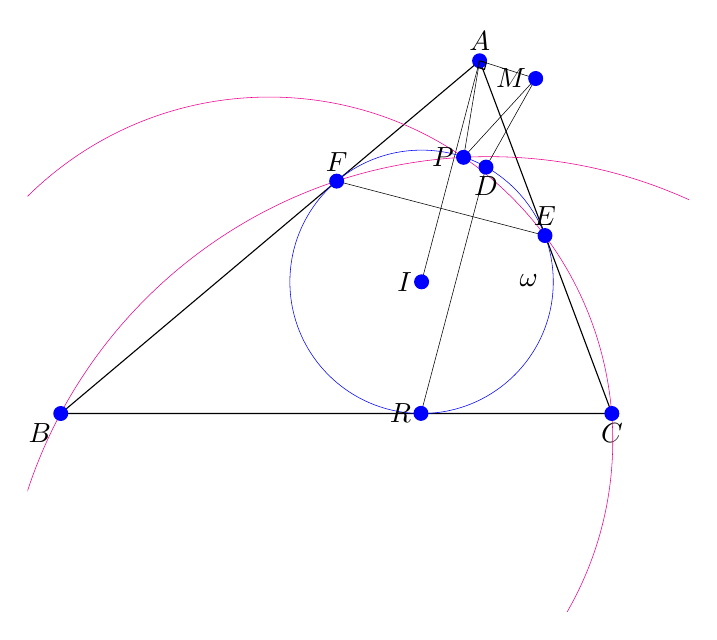
\begin{tikzpicture}[scale=1.4]
\tkzInit[xmin=-0.3,xmax=5.7,ymin=-1.8,ymax=3.5]
\tkzClip
\tkzSetUpPoint[size=5,fill=blue,color=blue]
\draw(0,0)coordinate(B) node[below left]{$B$}--(5,0)coordinate(C)node[below]{$C$}
--(3.8,3.2)coordinate(A)node[above]{$A$}--cycle;
\tkzInCenter(A,B,C)\tkzGetPoint{I}
\tkzDefPointBy[projection=onto B--C](I)\tkzGetPoint{D}
\tkzDefPointBy[projection=onto A--C](I)\tkzGetPoint{E}
\tkzDefPointBy[projection=onto A--B](I)\tkzGetPoint{F}
\tkzDrawCircle[draw=blue](I,D)
\tkzDefLine[perpendicular=through D](E,F)\tkzGetPoint{R'}
\tkzInterLC(D,R')(I,D)\tkzGetPoints{R}{D}
\tkzInterLC(A,R)(I,D)\tkzGetPoints{R}{P}
\tkzDrawSegments(E,F A,I D,R A,P)
\tkzCircumCenter(P,C,E)\tkzGetPoint{O1}
\tkzCircumCenter(P,B,F)\tkzGetPoint{O2}
\tkzInterCC(O1,P)(O2,P)\tkzGetPoints{P}{Q}
\tkzDrawCircle[draw=magenta](O1,P)\tkzDrawCircle[draw=magenta](O2,P)
\tkzInterLL(D,I)(P,Q)\tkzGetPoint{M}
\tkzDrawSegments(D,M A,M P,M)
\tkzLabelPoints[above](E,F)
\tkzLabelPoints[left](M,I,P,Q,R)
\tkzDrawPoints(A,B,C,D,E,F,P,Q,M,R,I)
\tkzMarkRightAngle[scale=0.5](M,A,I)
\tkzLabelCircle[left=2pt](I,D)(-60){$\omega$}
\node[below]at(D){$D$};
\end{tikzpicture}
\end{MYBOX}

\begin{MYBOX}[colbacktitle=green]{一道概率论练习题}
设$\{\xi_n\}$为独立同分布随机变量序列, $\{\xi_n\}$的分布列为$\begin{pmatrix}
-1&1\\0.5&0.5
\end{pmatrix},\eta_n=\sum_{k=1}^n\frac{\xi_k}{2^k}$.求证: $\{\eta_n\}$的分布收敛于$[-1,1]$上的均匀分布.
\tcblower
\begin{proof}
首先$\xi_k$的特征函数为
\[\varphi_{\xi_k}(t)=\mathbb E(\mathrm e^{\mathrm i\mskip3mu t\xi_k})=\frac12(\mathrm e^{\mathrm i\mskip3mu t}+\mathrm e^{-\mathrm i\mskip3mu t})=\cos t.\]
因此$\eta_n=\sum_{k=1}^n\frac{\xi_k}{2^k}$的特征函数为
\[\varphi_{\eta_n}(t)=\prod_{k=1}^n\varphi_{\xi_k}\left(\frac{t}{2^k}\right)=\prod_{k=1}^n
\cos\frac{t}{2^k}.\]
利用熟知的极限公式$\lim_{n\to\infty}\prod_{k=1}^n\cos\frac{t}{2^k}=\begin{cases}
\frac{\sin t}t,&t\ne0\\
1,&t=0
\end{cases}$,这刚好就是$[-1,1]$上均匀分布的特征函数,因此$\{\eta_n\}$的分布收敛于$[-1,1]$上的均匀分布.
\end{proof}
\end{MYBOX}
\begin{MYBOX}[colbacktitle=magenta]{一道线代练习题}
设$A,B$均为$n$阶实对称矩阵, 且$A$为非零半正定矩阵, $B$为正定矩阵,证明: $|A+B|>|B|$.
\tcblower
\begin{proof}
待证式等价于$|B^{-1}|\,|A+B|=|B^{-1}A+I|>1$.设$\lambda$为$B^{-1}A$的任一特征值,对应的特征向量为$x$,则$B^{-1}Ax=\lambda x$,即$Ax=\lambda Bx$,于是$x^{\mathrm T}Ax=\lambda x^{\mathrm T}Bx$,那么由条件可知$\lambda=\frac{x^{\mathrm T}Ax}{x^{\mathrm T}Bx}\ge0$.且由于$A$为非零矩阵,那么至少有一个特征值$\lambda\ne0$,于是$B^{-1}A+I$的所有特征值都不小于$1$,且至少有一个特征值严格大于$1$,于是$|B^{-1}|\,|A+B|=|B^{-1}A+I|>1$,得证.
\end{proof}
\end{MYBOX}
\begin{MYBOX}[colbacktitle=blue]{一道小思考题}
已知函数$f(x)$在$(0,1)$内可导,且满足$f'(x)\le \frac1{\sqrt x},x\in(0,1)$,问$f(x)$在$(0,1)$上是否有界?
\end{MYBOX}

\setcounter{example}{0}
\begin{MYBOX}[colbacktitle=blue]{纠正一道最近频繁问及的错题}
俗话说,好题不出门,坑题传千里.最近,很多qq群都在传一道错误的中值定理证明题如下:

设$f(x)$在$[a,b]$上有二阶连续导数,且$f(a)=f(b)=0$,证明存在$\xi\in[a.b]$,使得$\int_a^bf(x)\,\mathrm dx=\frac{f''(\xi)}6(b-a)^3$.

直接取反例$f(x)=x(1-x),[a,b]=[0,1]$可知题目是错的,正确的题目应当是
\begin{example}
设$f(x)$在$[a,b]$上有二阶连续导数,且$f(a)=f(b)=0$,证明存在$\xi\in[a.b]$,使得$\int_a^bf(x)\,\mathrm dx=-\frac{f''(\xi)}{12}(b-a)^3$.进一步,我们需要说明,这里的$-\frac1{12}$其实就是最佳系数.
\end{example}
\begin{proof}
首先注意到由分部积分可得
\[\int_a^bf(x)\,\mathrm dx=-\frac12\int_a^bf''(x)(x-a)(b-x)\,\mathrm dx,\]
然后由积分中值定理得
\[\int_a^bf(x)\,\mathrm dx=-\frac12f''(\xi)\int_a^b(x-a)(b-x)\,\mathrm dx=-\frac{f''(\xi)}{12}(b-a)^3.\]
事实上通过以上过程,我们证明了
\[\left|\int_a^bf(x)\,\mathrm dx\right|\le \frac{M}{12}(b-a)^3,\quad M=\max_{a\le x\le b}|f''(x)|,\]
而且取$f(x)=(x-a)(b-x)$可以取等,所以系数$-\frac1{12}$是最佳的.
\end{proof}

纵观上述证明,我们利用到了$f''(x)$的可积性,也就是题目给定了$f''(x)$的连续性.但是根据Darboux定理可知$f''(x)$的介值性不依赖于它的连续性,于是,我们可以将题目中的二阶连续可导改为二阶可导,结论照样成立,但证明的难度会变大.

令$K=-\frac{12}{(b-a)^3}\int_a^bf(x)\,\mathrm dx$,用反证法,假设不存在$\xi$使得$f''(\xi)=K$成立,根据Darboux定理有$f''(x)>K$或者$f''(x)<K$恒成立.不妨设$f''(x)>K,x\in[a,b]$.那么由Taylor公式可得
\[0=f(a)=f(x)+f'(x)(a-x)+\frac{f''(\eta_x)}2(a-x)^2,\]
则
\begin{align*}
\int_a^b[f(x)+f'(x)(a-x)]\,\mathrm dx&=2\int_a^bf(x)\,\mathrm dx\\
&=-\int_a^b\frac{f''(\eta_x)}2(a-x)^2\,\mathrm dx<-\frac K2\int_a^b(a-x)^2\,\mathrm dx\\
&=-\frac K{6}(b-a)^3=2\int_a^bf(x)\,\mathrm dx,
\end{align*}
矛盾,因此原结论成立.
\end{MYBOX}

\begin{MYBOX}[colbacktitle=blue]{再谈行列式降阶公式}\setlength{\parindent}{2em}
在两年前的博文中,其实我们已经很详细探讨过矩阵$AB$与$BA$的关系,最近在上课的时候又碰到类似的问题,我们简单介绍一下.
\begin{theorem}[行列式降阶公式]
设$A_{m\times n},B_{n\times m}$,则$\lambda^n|\lambda E_m\pm AB|=\lambda^n|\lambda E\pm BA|$.
\end{theorem}
\begin{proof}
在等式
\[\begin{pmatrix}
E_n&O\\A&E_m
\end{pmatrix}\begin{pmatrix}
\lambda E_n&B\\O&\lambda E_m\pm AB
\end{pmatrix}\begin{pmatrix}
E_n&O\\-A&E_m
\end{pmatrix}=\begin{pmatrix}
\lambda E_n\pm BA&B\\O&\lambda E_m
\end{pmatrix}\]
两边取行列式即可得到.
\end{proof}
对于数学系的同学这个公式应用还是非常广的,比如下面的行列式:
\[
\left| \begin{matrix}
	\lambda +a_1b_1&		a_1b_2&		\cdots&		a_1b_n\\
	a_2b_1&		\lambda+a_2b_2&		\cdots&		a_2b_n\\
	\vdots&		\vdots&		\ddots&		\vdots\\
	a_nb_1&		a_nb_2&		\cdots&		\lambda+a_nb_n\\
\end{matrix} \right|
\]
记$\alpha=(a_1,\cdots,a_n)^{\mathrm T},\beta=(b_1,\cdots,b_n)^{\mathrm T}$,那么有$|\lambda E_n+\alpha\beta^{\mathrm T}|=|\lambda+\beta\alpha^{\mathrm T}|=\lambda+a_1b_1+\cdots+a_nb_n$.

对于非数学类的学生而言,更多的是在$n=m$的条件下应用.行列式的降阶公式其实等价于$\lambda^n\varphi_{AB}(\lambda)=\lambda^m\varphi_m(BA)$,也就是$AB$与$BA$的特征多项式其实就相差一个因子$\lambda^{n-m}$,这说明$AB$与$BA$的所有非零特征值连同其重数都是相同的.由迹与特征值的关系可知$\tr(AB)=\tr(BA)$.事实上,令$A_{m\times n}=(a_{ij}),B=(b_{ji})$,则$\tr(AB)=\tr(BA)=\sum_{i=1}^m\sum_{j=1}^na_{ij}b_{ji}$.应用这个性质可知$\tr(A^{\mathrm T}A)=\sum_{i,j=1}^na_{ij}^2$,于是$A=O\Leftrightarrow \tr(A^{\mathrm T}A)=0$.比如我们可以解决一道很简单的征解题: 如果$A^{\mathrm T}A=A^2$,则$A=A^{\mathrm T}$.这只需证明$\tr(A-A^{\mathrm T})(A-A^{\mathrm T})^{\mathrm T}=0$即可,显然.

最后我们看一个非数类的一道考题:设$A,B$都是$n$阶方阵,已知$E+AB$可逆,证明$E+BA$可逆.
\begin{proof}
这道题利用降阶公式直接秒杀,而原题则是构造一些列的方程组,写了一大堆.不过这里我们用另一种写法, 先证明$AB$与$BA$具有相同的非零特征值: 设$ABX=\lambda X,\lambda\ne0,X\ne\boldsymbol 0$,则$BX\ne\boldsymbol0$,于是$(BA)BX=\lambda BX$,这说明$AB$的非零特征值都是$BA$的非零特征值,反之也对.那么$E+AB$可逆说明$AB$没有特征值$-1$,于是$BA$也没有特征值$-1$, 即$E+BA$可逆.
\end{proof}
\end{MYBOX}
\begin{MYBOX}[colbacktitle=blue]{四道颇有意思的不定积分}\setlength{\parindent}{2em}
最近在贴吧看到一道不定积分题如下
\[\int\frac{x\sin x}{(x+\sin x)^2}\,\mathrm dx.\]
这题原则上讲,还是小有难度的,然后我用MMA简单算了一下,确实是有初等原函数的.像这种构造的函数,能够有初等原函数确实不容易,同时我还发现,下面几个积分都是一样的
\[\int\frac{x\sin x}{(x+\sin x)^2}\,\mathrm dx,\int\frac{x\sin x}{(x-\sin x)^2}\,\mathrm dx,\int\frac{x\cos x}{(x+\cos x)^2}\,\mathrm dx,\int\frac{x\cos x}{(x-\cos x)^2}\,\mathrm dx.\]
这里我们给出最后一个积分的计算,其他都类似.
\begin{align*}
\int\frac{x\cos x}{(x-\cos x)^2}\,\mathrm dx&=\int{\frac{x\cos x}{1+\sin x}\frac{1+\sin x}{\left( x-\cos x \right) ^2}\,\mathrm{d}x}\\
&=-\int{\frac{x\cos x}{1+\sin x}\,\text{d}\left( \frac{1}{x-\cos x} \right)}\\
&=-\frac{x\cos x}{\left( 1+\sin x \right) \left( x-\cos x \right)}+\int{\frac{1}{x-\cos x}\,\text{d}\left( \frac{x\cos x}{1+\sin x} \right)}\\
&=-\frac{x\cos x}{\left( 1+\sin x \right) \left( x-\cos x \right)}+\int{\frac{1}{x-\cos x}\frac{-x+\cos x}{1+\sin x}\,\text{d}x}\\
&=-\frac{x\cos x}{\left( 1+\sin x \right) \left( x-\cos x \right)}+\frac{\cos x}{1+\sin x}+C\\
&=-\frac{\cos ^2x}{\left( x-\cos x \right) \left( 1+\sin x \right)}+C=\frac{\sin x-1}{x-\cos x}+C.
\end{align*}
\end{MYBOX}
\begin{MYBOX}[colbacktitle=blue]{2019年全国高中数学联赛一试A卷}
\textbf{一、填空题: 本大题共8小题,每小题8分,满分64分.}
\begin{enumerate}
\item 已知正实数$a$满足$a^a=(9a)^{8a}$,则$\log_a(3a)$的值为\kong.\\
答案: $\frac9{16}$.
\item 若实数集合$\{1,2,3,x\}$的最大元素与最小元素之差等于该集合的所有元素之和,则$x$的值为\kong.\\
答案: $-\frac32$.
\item 平面直角坐标系中, $\OR{e}$是单位向量,向量$\OR{a}$满足$\OR{a}\cdot\OR{e}=2$,且$|\OR{a}|^2\le5|\OR{a}+t\OR{e}|$对任意实数$t$成立,则$|\OR{a}|$的取值范围是\kong.\\
答案: $\left[\sqrt5,2\sqrt5\right]$.
\item 设$A,B$为椭圆$\Gamma$的长轴顶点, $E,F$为$\Gamma$的两个交点, $|AB|=4,|AF|=2+\sqrt3,P$为$\Gamma$上一点,满足$|PE|\cdot|PF|=2$,则$\triangle PEF$的面积为\kong.\\
答案: $1$.
\item 在$1,2,3,\cdots,10$中随机选出一个数$a$,在$-1,-2,\cdots,-10$中随机选出一个数$b$,则$a^2+b$被$3$整除的概率为\kong.\\
答案: $\frac{37}{100}$.
\item 对任意闭区间$I$,用$M_I$表示函数$y=\sin x$在$I$上的最大值,若正数$a$满足$M_{[0,a]}=2M_{[a,2a]}$,则$a$的值为\kong.\\
答案: $\frac56\pi$或$\frac{13}{12}\pi$.
\item 正方体$ABCD-EFGH$的一个截面经过顶点$A,C$及棱$EF$上一点$K$,且将正方体分成体积比为$3:1$的两部分,则$\frac{EK}{KF}$的值为\kong.\\
答案: $\sqrt3$.
\item 将$6$个数$2,0,1,9,20,19$按任意次序排成一行,拼成一个$8$位数(首位不为$0$),则产生的不同的$8$位数的个数为\kong.\\
答案: $498$.
\end{enumerate}
\textbf{二、解答题: 本大题共3小题,满分56分.}
\begin{enumerate}
\setcounter{enumi}{8}
\item ({\kaishu 本题满分16分})在$\triangle ABC$中, $BC=a,CA=b,AB=c$.若$b$是$a$与$c$的等比中项,且$\sin A$是$\sin(B-A)$与$\sin C$的等差中项,求$\cos B$的值.\\
答案: $\frac{\sqrt5-1}2$.
\item 在平面直角坐标系$xOy$中,圆$\Omega$与抛物线$\Gamma :y^2=4x$恰有一个公共点,且圆$\Omega$与$x$轴相切于$\Gamma$的焦点$F$.求圆$\Omega$的半径.\\
答案: $\frac{4\sqrt3}9$.
\item 称一个复数列$\{z_n\}$为``有趣的'',若$|z_1|=1$,且对任意正整数$n$,均有$4z_{n+1}^2+2z_nz_{n+1}+z_n^2=0$.求最大的常数$C$,使得对一切有趣的数列$\{z_n\}$及任意正整数$m$,均有$|z_1+z_2+\cdots+z_m|\ge C$.\\
答案: $\frac{\sqrt3}3$.
\end{enumerate}
\end{MYBOX}
\begin{MYBOX}[colbacktitle=blue]{2019年全国高中数学联赛二试A卷}
\textbf{一}、({\kaishu 本题满分40分})如图 \ref{fig1} ,在锐角$\triangle ABC$中, $M$是$BC$边的中点.点$P$在$\triangle ABC$内,使得$AP$平分$\angle BAC$,直线$MP$与$\triangle ABP,\triangle ACP$的外接圆分别相交于不同于点$P$的两点$D$、$E$.证明: 若$DE=MP$,则$BC=2BP$.
\begin{figure}[H]\tikzset{inner sep=2.5pt}\captionsetup{labelsep=none}
\begin{minipage}[t]{0.5\linewidth}
\centering
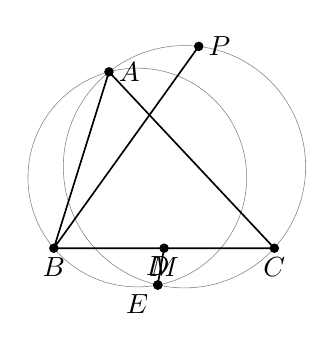
\begin{tikzpicture}[scale=0.7]
\tkzDefPoints{0/0/B,4/0/C,1/3.2/A}
\tkzDefMidPoint(B,C)\tkzGetPoint{M}
\tkzInCenter(A,B,C)\tkzGetPoint{I}
\tkzInterLC(A,I)(B,M)\tkzGetFirstPoint{P}
\tkzCircumCenter(A,B,P)\tkzGetPoint{O1}
\tkzCircumCenter(A,C,P)\tkzGetPoint{O2}
\tkzInterLC(P,M)(O1,A)\tkzGetPoints{D}{P}
\tkzInterLC(P,M)(O2,A)\tkzGetPoints{P}{E}
\tkzDrawCircle(O1,A)\tkzDrawCircle(O2,A)

\draw[semithick](A)--(B)--(C)--cycle(M)--(D)(B)--(P);
\tkzLabelPoints[above](D)
\tkzLabelPoints[right](A,P)
\tkzLabelPoints[below](B,M,C)
\tkzLabelPoints[below left](E)
\tkzDrawPoints[size=3,fill=black](A,B,C,M,P,D,E)
\end{tikzpicture}
\caption{}
\label{fig1}
\end{minipage}%
\begin{minipage}[t]{0.5\linewidth}
\centering
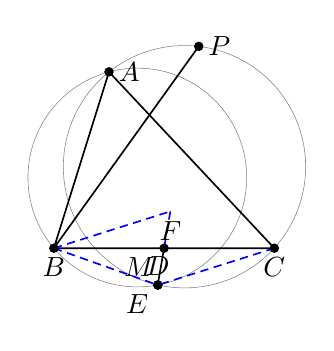
\begin{tikzpicture}[scale=0.7]
\tkzDefPoints{0/0/B,4/0/C,1/3.2/A}
\tkzDefMidPoint(B,C)\tkzGetPoint{M}
\tkzInCenter(A,B,C)\tkzGetPoint{I}
\tkzInterLC(A,I)(B,M)\tkzGetFirstPoint{P}
\tkzCircumCenter(A,B,P)\tkzGetPoint{O1}
\tkzCircumCenter(A,C,P)\tkzGetPoint{O2}
\tkzInterLC(P,M)(O1,A)\tkzGetPoints{D}{P}
\tkzInterLC(P,M)(O2,A)\tkzGetPoints{P}{E}
\tkzDrawCircle(O1,A)\tkzDrawCircle(O2,A)
\draw[semithick,](A)--(B)--(C)--cycle(M)--(D)(B)--(P);
\tkzDefLine[parallel=through B](E,C)
\tkzGetPoint{F}

\draw[semithick,blue,densely dashed](B)--(F)(F)--(M)(B)--(D)(C)--(E);
\tkzLabelPoints[above](D)
\tkzLabelPoints[right](A,P)
\tkzLabelPoints[below](B,C,F)
\tkzLabelPoints[below left](E,M)
\tkzDrawPoints[size=3,fill=black](A,B,C,M,P,D,E)
\end{tikzpicture}
\caption{}\label{fig2}
\end{minipage}
\end{figure}
\begin{proof}
如图 \ref{fig2}, 延长$PM$到点$F$,使得$MF=ME$,连接$BF,BD,CE$.由条件可知
\[\angle BDP=\angle BAP=\angle CAP=\angle CEP=\angle CEM.\]
因为$BM=CM$且$EM=FM$,所以$BF=CE$且$BF\pxx CE$,于是$\angle F=\angle CEM=\angle BDP$,进而$BD=BF$.又$DE=MP$,故$DP=EM=FM$.于是在等腰$\triangle ABC$中,由对称性得$BP=BM$,从而$BC=2BM=2BP$.
\end{proof}
\textbf{二}、({\kaishu 本题满分40分})设整数$a_1,a_2,\cdots,a_{2019}$满足$1=a_1\le a_2\le\cdots\le a_{2019}=99$.记
\[f=(a_1^2+a_2^2+\cdots+a_{2019}^2)-(a_1a_3+a_2a_4+a_3a_5+\cdots+a_{2017}a_{2019}),\]
求$f$的最小值$f_0$,并确定使$f=f_0$成立的数组$(a_1,a_2,\cdots,a_{2019})$的个数.\\
答案: $f_0=7400$,使$f=f_0$成立的数组$(a_1,a_2,\cdots,a_{2019})$的个数为$\textrm C_{1968}^{48}$.

\textbf{三}、({\kaishu 本题满分50分})设$m$为正整数, $|m|\ge2$.整数列$a_1,a_2,\cdots,$满足: $a_1,a_2$不全为零,且对任意正整数$n$, 均有$a_{n+2}=a_{n+1}-ma_n$.证明: 若存在整数$r,s\,(r>s\ge2)$使得$a_r=a_s=a_1$,则$r-s\ge|m|$.\\
证明: 略.

\textbf{四}、({\kaishu 本题满分50分})设$V$是空间中$2019$个点构成的集合,其中任意四点不共勉.某些点之间连有线段,记$E$为这些线段构成的集合.试求最小的正整数$n$,满足条件: 若$E$至少有$n$个元素,则$E$一定含有$908$个二元子集,其中每个二元子集中的两条线段有公共端点,且任意两个二元子集的交为空集.\\
答案: 2795.
\end{MYBOX}
\begin{MYBOX}[colbacktitle=cyan]{几个有趣的结果}
\begin{gather*}
\int_{-\infty}^{+\infty}{\frac{\sin x}{x}\text{d}x}=\sum_{n=-\infty}^{\infty}{\frac{\sin n}{n}}=\pi,\\
\int_{-\infty}^{+\infty}{\left( \frac{\sin x}{x} \right) ^2\text{d}x}=\sum_{n=-\infty}^{\infty}{\left( \frac{\sin n}{n} \right) ^2}=\pi,\\
\int_{-\infty}^{+\infty}{\left( \frac{\sin x}{x} \right) ^3\text{d}x}=\sum_{n=-\infty}^{\infty}{\left( \frac{\sin n}{n} \right) ^3}=\frac{3\pi}{4},\\
\int_{-\infty}^{+\infty}{\left( \frac{\sin x}{x} \right) ^4\text{d}x}=\sum_{n=-\infty}^{\infty}{\left( \frac{\sin n}{n} \right) ^4}=\frac{2\pi}{3},\\
\int_{-\infty}^{+\infty}{\left( \frac{\sin x}{x} \right) ^5\text{d}x}=\sum_{n=-\infty}^{\infty}{\left( \frac{\sin n}{n} \right) ^5}=\frac{115\pi}{192},\\
\int_{-\infty}^{+\infty}{\left( \frac{\sin x}{x} \right) ^6\text{d}x}=\sum_{n=-\infty}^{\infty}{\left( \frac{\sin n}{n} \right) ^6}=\frac{11\pi}{20}.
\end{gather*}
数值结果显示,上述等式从7次方开始就不再成立了.
\end{MYBOX}
\begin{MYBOX}[colbacktitle=cyan]{解答一道贴吧级数题}
今天逛了一下贴吧,看到一道级数题如下:
\[\sum_{k=1}^\infty\left[k^2\ln\left(1-\frac1{4k^2}\right)+\frac14\right].\]
好久没做这种题了,还有点手生了.解答此题我们需要利用$\zeta$函数的母函数与$\ln\sin x$的傅里叶级数:
\[\sum_{n=1}^\infty\zeta(2n)x^{2n}=\frac{1-\pi x\cot\pi x}2,\quad\ln\sin x=-\ln2-\sum_{n=1}^\infty\frac{\cos2nx}n.\]
下面就是计算了.
\begin{align*}
\sum_{k=1}^{\infty}{\left[ k^2\ln \left( 1-\frac{1}{4k^2} \right) +\frac{1}{4} \right]}&=\sum_{k=1}^{\infty}{\left[ -k^2\sum_{n=1}^{\infty}{\frac{1}{n4^nk^{2n}}}+\frac{1}{4} \right]}\\
&=-\sum_{n=2}^{\infty}{\frac{1}{n4^n}\sum_{k=1}^{\infty}{\frac{1}{k^{2n-2}}}}=-\sum_{n=2}^{\infty}{\frac{\zeta \left( 2n-2 \right)}{n\cdot 4^n}}\\
&=-\sum_{n=1}^{\infty}{\frac{\zeta \left( 2n \right)}{\left( n+1 \right) 2^{2n+2}}}=-2\sum_{n=1}^{\infty}{\zeta \left( 2n \right) \int_0^{\frac{1}{2}}{x^{2n+1}\text{d}x}}\\
&=-2\int_0^{\frac{1}{2}}{\sum_{n=1}^{\infty}{\zeta \left( 2n \right) x^{2n+1}}\text{d}x}=\int_0^{\frac{1}{2}}{\left( \pi x^2\cot \pi x-x \right) \text{d}x}\\
&=\int_0^{\frac{1}{2}}{\pi x^2\cot \pi x\text{d}x}-\frac{1}{8}=\frac{1}{\pi ^2}\int_0^{\frac{\pi}{2}}{t^2\cot t\text{d}t}-\frac{1}{8}\\
&=\frac{\ln2}4-\frac7{8\pi^2}\zeta(3)-\frac18.
\end{align*}
其中
\begin{align*}
\int_0^{\frac{\pi}{2}}{t^2\cot t\text{d}t}&=\int_0^{\frac{\pi}{2}}{t^2\text{d}\left( \ln\sin t \right)}=-2\int_0^{\frac{\pi}{2}}{t\ln\sin t\text{d}t}\\
&=2\int_0^{\frac{\pi}{2}}{t\ln 2\text{d}t}-2\sum_{n=1}^{\infty}{\frac{1}{n}}\int_0^{\frac{\pi}{2}}{t\cos 2nt\text{d}t}\\
&=\frac{\pi ^2}{4}\ln 2-2\sum_{n=1}^{\infty}{\frac{-1+\left( -1 \right) ^n}{4n^2}}=\frac{\pi ^2}{4}\ln 2-\frac{7}{8}\zeta \left( 3 \right).
\end{align*}

\end{MYBOX}

\begin{MYBOX}[colbacktitle=blue]{美国数学月刊征解题12143}
求
\[\lim_{n\to\infty}\sum_{k=1}^n\left(\frac kn\right)^k.\]
\begin{solve}
首先$\sum_{k=1}^n\left(\frac kn\right)^k=\sum_{k=0}^{n-1}\left(\frac{n-k}n\right)^{n-k}$,对每个固定的$k$,有
\[\lim_{n\to\infty}\left(\frac{n-k}n\right)^{n-k}
=\lim_{n\to\infty}\left(1-\frac kn\right)^{n-k}=\ee^{-k}.\]
因此
\[
\varlimsup_{n\rightarrow \infty}\sum_{k=0}^{n-1}{\left( \frac{n-k}{n} \right) ^{n-k}}\leqslant \sum_{k=0}^{\infty}\varlimsup_{n\rightarrow \infty}\left( \frac{n-k}{n} \right) ^{n-k}=\sum_{k=0}^{\infty}{\text{e}^{-k}}=\frac{\text{e}}{\text{e}-1}.
\]
另一方面,对每个固定的$m$,
\[
\lim_{n\rightarrow \infty} \sum_{k=0}^m{\left( \frac{n-k}{n} \right) ^k}=\sum_{k=0}^m{\lim_{n\rightarrow \infty}}\left( \frac{n-k}{n} \right) ^k=\sum_{k=0}^m{\text{e}^{-k}}=\frac{\text{e}-\text{e}^{-m}}{\text{e}-1},
\]
令$m\to\infty$可知$\varliminf_{n\to\infty}\sum_{k=0}^{n-1}{\left( \frac{n-k}{n} \right) ^k}\geqslant \lim_{m\rightarrow \infty} \frac{\text{e}-\text{e}^{-m}}{\text{e}-1}=\frac{\text{e}}{\text{e}-1}$,因此所求的极限值就是$\frac{\ee}{\ee-1}$.
\end{solve}
\end{MYBOX}

\begin{MYBOX}[colbacktitle=red]{美国数学月刊征解题12145}
证明:
\[\int_0^{\infty}\frac{\cos (t)\sin\left(\sqrt{1+t^2}\right)}{\sqrt{1+t^2}}\mathrm dt=\frac\pi4.\]
\begin{Proof}
\begin{align*}
\int_0^{\infty}\frac{\cos (t)\sin\left(\sqrt{1+t^2}\right)}{\sqrt{1+t^2}}\mathrm dt
&\xlongequal{t=\sinh x}\int_0^{\infty}{\frac{\cos \left( \sinh x \right) \sin \left( \cosh x \right)}{\cosh x}\cosh x\text{d}x}\\
&=\frac{1}{2}\int_0^{\infty}{\bigl( \sin \left( \cosh x+\sinh x \right) +\sin \left( \cosh x-\sinh x \right) \bigr) \text{d}x}\\
&=\frac{1}{4}\int_{-\infty}^{\infty}{\bigl( \sin \left( \text{e}^x \right) +\sin \left( \text{e}^{-x} \right) \bigr) \text{d}x}\\
&=\frac{1}{2}\int_{-\infty}^{\infty}{\sin \left( \text{e}^x \right) \text{d}x}=\frac{1}{2}\int_0^{\infty}{\frac{\sin u}{u}\text{d}u}\\
&=\frac{\pi}{4}.
\end{align*}
\end{Proof}
\end{MYBOX}

\begin{MYBOX}[colbacktitle=blue]{2019年12月8日美国普特南大学生数学竞赛题}
设
\[
a_n=\sum_{k=1}^{n-1}{\frac{\sin \left( \frac{\left( 2k-1 \right)}{2n}\pi \right)}{\cos ^2\left( \frac{\left( k-1 \right) \pi}{2n} \right) \cos ^2\left( \frac{k\pi}{2n} \right)}},
\]
求$\lim_{n\to\infty}\frac{a_n}{n^3}$.
\begin{solve}
首先我们有三角恒等式
\begin{align*}
\cos^2\alpha-\cos^2\beta&=(\cos\alpha+\cos\beta)(\cos\alpha-\cos\beta)\\
&=2\cos\frac{\alpha+\beta}2\cos\frac{\alpha-\beta}2\cdot2\sin\frac{\alpha+\beta}2
\sin\frac{\beta-\alpha}2\\
&=\sin(\beta-\alpha)\sin(\beta+\alpha).
\end{align*}
于是
\begin{align*}
a_n&=\frac{1}{\sin \frac{\pi}{2n}}\sum_{k=1}^{n-1}{\frac{\sin \frac{\pi}{2n}\sin \left( \frac{\left( 2k-1 \right)}{2n}\pi \right)}{\cos ^2\left( \frac{\left( k-1 \right) \pi}{2n} \right) \cos ^2\left( \frac{k\pi}{2n} \right)}}\\
&=\frac{1}{\sin \frac{\pi}{2n}}\sum_{k=1}^{n-1}{\frac{\cos ^2\left( \frac{\left( k-1 \right) \pi}{2n} \right) -\cos ^2\left( \frac{k\pi}{2n} \right)}{\cos ^2\left( \frac{\left( k-1 \right) \pi}{2n} \right) \cos ^2\left( \frac{k\pi}{2n} \right)}}\\
&=\frac{1}{\sin \frac{\pi}{2n}}\sum_{k=1}^{n-1}{\left( \frac{1}{\cos ^2\left( \frac{k\pi}{2n} \right)}-\frac{1}{\cos ^2\left( \frac{\left( k-1 \right) \pi}{2n} \right)} \right)}\\
&=\frac{1}{\sin \frac{\pi}{2n}}\left( \frac{1}{\cos ^2\frac{n-1}{2n}\pi}-1 \right)=\frac{\sin ^2\frac{n-1}{2n}\pi}{\sin \frac{\pi}{2n}\cos ^2\frac{n-1}{2n}\pi}\\
&=\frac{\sin ^2\frac{n-1}{2n}\pi}{\sin ^3\frac{\pi}{2n}}.
\end{align*}
于是
\[
\lim_{n\rightarrow \infty} \frac{a_n}{n^3}=\lim_{n\rightarrow \infty} \frac{\sin ^2\frac{n-1}{2n}\pi}{n^3\sin ^3\frac{\pi}{2n}}=\left( \frac{2}{\pi} \right) ^3=\frac{8}{\pi ^3}
\]
\end{solve}
\end{MYBOX}
\begin{MYBOX}[colbacktitle=blue]{Ovidiu Furdui的一道征解题}
求出所有的函数$f:\mathbb R\to\mathbb R$,使得其满足如下函数方程:
\[f(-x)=1+\int_0^x\sin(t)f(x-t)\,\mathrm dt.\]
\tcblower
\begin{solve}
由所给的等式可知$f(x)$具有足够可导性, 且$f(0)=1$.换元$x-t=u$可得
\begin{align*}
f\left( -x \right) &=1+\int_0^x{\sin \left( x-u \right) f\left( u \right) \text{d}u}\\
&=1+\boxed{\sin x\int_0^x{f\left( u \right) \cos u\text{d}u}-\cos x\int_0^x{f\left( u \right) \sin u\text{d}u}}.
\end{align*}
等式两边求导得
\[
-f'\left( -x \right) =\cos x\int_0^x{f\left( u \right) \cos u\text{d}u}+\sin x\int_0^x{f\left( u \right) \sin u\text{d}u},
\]
于是$f'(0)=0$.再求导得
\begin{align*}
f''\left( -x \right) &=\boxed{-\sin x\int_0^x{f\left( u \right) \cos u\text{d}u}+\cos x\int_0^x{f\left( u \right) \sin u\text{d}u}}+f\left( x \right)\\
&=f(x)-f(-x)+1.
\end{align*}
于是$f''(0)=f(0)=1$,且$f''(x)=f(-x)-f(x)+1=2-f''(-x)$. 等式两边再继续求导得
\begin{gather*}
-f'''\left( -x \right) =f'\left( x \right) +f'\left( -x \right) ,\\
f^{\left( 4 \right)}\left( -x \right) =f''\left( x \right) -f''\left( -x \right) =2-2f''\left( -x \right),
\end{gather*}
即$f'''(0)=-1,f^{(4)}(x)+2f''(x)=1$,解此四阶常系数线性微分方程可得$f(x)=\frac12x^2+1$.
\end{solve}
\end{MYBOX}

\begin{MYBOX}[colbacktitle=blue]{北京大学2020年考研数学分析第三题解答}
已知$f(x)$在$[0,1]$上连续,单调增加且$f(x)\ge0$. 记
\[s=\frac{\int_0^1xf(x)\,\mathrm dx}{\int_0^1f(x)\,\mathrm dx}.\]
\begin{enumerate}[(1)]
\item 证明$s\ge\frac12$.
\item 比较$\int_0^sf(x)\,\mathrm dx$与$\int_s^1f(x)\,\mathrm dx$的大小.(可以用物理或几何直觉)
\end{enumerate}
\tcblower
\begin{Proof}
这题我很早前在贴吧见过解答. 第一问属于比较简单的问题,第二问则是非常难,当然,如果是只要猜答案,应该时可以用直觉猜出来的,我们给出严格的证明. 对于这样的积分不等式问题, 函数的连续性条件往往是多余的, 这里直接去掉这个条件进行证明.

(1) 由Chebyshev不等式得
\[\int_0^1xf(x)\,\mathrm dx\ge\int_0^1x\,\mathrm dx\int_0^1f(x)\,\mathrm dx=\frac12\int_0^1f(x)\,\mathrm dx.\]

(2) 我们先猜一下答案, 考虑一根在区间$[0,1]$上的密度为$f(x)$的棒, $s$就是其重心所在的位置, 重心的左右两侧保持杠杆平衡, 也就是满足重力与重力臂的乘积相等, $F_1l_1=F_2l_2$. $s$的左边更长, 其力臂更长,对应的重力小一些, 也就是质量轻一点,因此$\int_0^sf(x)\,\mathrm dx\le\int_s^1f(x)\,\mathrm dx$.下面我们来严格证明:
\[\int_0^sf(x)\,\mathrm dx\le\int_s^1f(x)\,\mathrm dx.\]
令$F(x)=\int_0^xf(t)\,\mathrm dt$, 由题意知$F(x)$是单调递增的(下)凸函数, 为方便,我们不妨假定
\[F(1)=\int_0^1f(t)\,\mathrm dt=1.\]
于是有
\[s=\int_0^1xf(x)\,\mathrm dx=1-\int_0^1F(x)\,\mathrm dx,\]
那么原不等式则等价于
\[F(s)\le 1-F(s).\]
等价于证明$f(s)\le\frac12$. 那么由Jensen不等式得
\begin{align*}
F(s)&=F\left(1-\int_0^1F(x)\,\mathrm dx\right)=F\left(\int_0^1\big(1-F(x)\big)\,\mathrm dx\right)\\
&=\int_0^1F\left(\int_x^1f(t)\,\mathrm dt\right)\le\int_0^1\int_x^1F\big(f(t)\big)\,\mathrm dt\mathrm dx\\
&\le\int_0^1\int_x^11\mathrm dt\mathrm dx=\frac12.
\end{align*}

\end{Proof}
\end{MYBOX}

\begin{MYBOX}[colbacktitle=blue]{College Mathematics Journal期刊征解题1167解答}
证明以下等式:
\begin{enumerate}
  \item \label{eq1} $\sum_{n=0}^\infty\binom{2n}n\frac1{4^n(n+1)}=2$,
  \item \label{eq2} $\sum_{n=0}^\infty\binom{2n}n\frac1{4^n(n+1)^2}=4-4\ln2$,
  \item \label{eq3} $\sum_{n=0}^\infty\binom{2n}n\frac1{4^n(n+1)^3}=4\ln^22-8\ln2-
  \frac{\pi^2}3+8$.
\end{enumerate}
\tcblower
\begin{Proof}
首先我们有
\[\arcsin x=\sum_{n=0}^\infty\binom{2n}n\frac{x^n}{4^n}=\frac1{1-x}.\]
于是两边从$0$到$x$积分得
\[\sum_{n=0}^\infty\binom{2n}n\frac{x^{n+1}}{4^n(n+1)}=\int_0^x\frac{\mathrm dt}
{\sqrt{1-t}}=2-2\sqrt{1-x}.\]
取$x=1$得等式 \ref{eq1}. 等式两边除以$x$再从$0$到$x$积分得
\begin{align*}
\sum_{n=0}^\infty\binom{2n}n\frac{x^{n+1}}{4^n(n+1)^2}&=
\int_0^x\frac{2-2\sqrt{1-t}}t\mathrm dt\\
&=4-4\ln2+4\ln\left(1+\sqrt{1-x}\right)-4\sqrt{1-x}.
\end{align*}
取$x=1$得等式 \ref{eq2}. 两边再除以$x$,再从$0$到$1$积分得
\begin{align*}
\sum_{n=0}^\infty\binom{2n}n\frac{1}{4^n(n+1)^3}&=
4\int_0^1\frac{1-\ln2+\ln\left(1+\sqrt{1-x}\right)-\sqrt{1-x}}x\mathrm dx\\
&=4\ln^22-8\ln2-\frac{\pi^2}3+8.
\end{align*}
其中
\begin{gather*}
\int_0^1\frac{1-\sqrt{1-x}}x\mathrm dx
=\int_0^{\frac\pi2}\frac{1-\cos t}{\sin^2t}2\sin t\cos t\mathrm dt=2-2\ln2.\\
\int_0^1\frac{\ln\left(1+\sqrt{1-x}\right)-\ln2}x\mathrm dx=\ln^22-\frac{\pi^2}{12}.
\end{gather*}
其中最后一个积分参见我的积分级数文档34题.
\end{Proof}


\end{MYBOX}
\begin{MYBOX}[colbacktitle=blue]{解答李雅老师微博一题}
证明$\sin x+\sin\pi x$不是周期函数.
\tcblower
\begin{Proof}\parindent=2em
要证明这个问题,我们首先承认一个事实: $\pi$是一个无理数, 当然, $\pi$是无理数这个结论已经远远超出了本题的难度,我们姑且承认它.

反证法, 假定$T\ne0$是$f(x)=\sin x+\sin \pi x$的一个周期,那么$T$也是$f'(x)=\cos x+\pi\cos\pi x$的一个周期,于是
\[f'(0)=f'(T)\Rightarrow1+\pi=\cos T+\pi\cos\pi T.\]
因此有$\cos T=1,\pi\cos\pi T=\pi$,前者说明$T=2k_1\pi$,后者说明$\pi T=2k_2\pi$,这里$k_1,k_2$都是整数,从而$\pi=\frac{k_2}{k_1}$,这说明$\pi$是一个有理数,矛盾,因此$f(x)$不是周期函数.

关于这题,南京师范大学宣立新老师早期给过更一般的结论.
\end{Proof}
\end{MYBOX}
\newpage
\begin{MYBOX}[colbacktitle=blue]{一道不等式证明}
对实数$\lambda<\ee$, 证明
\[\int_0^{+\infty}\frac{\mathrm dz}{\ee^z-\lambda z}<\pi\sqrt{\frac2{\ee(\ee-\lambda)}}.\]
\tcblower
\begin{Proof}\parindent=2em
最近出现在贴吧的这个不等式相当火,当然难度相当的大.这题的不等式是非常sharp的, 当$\lambda\to\ee^-$时, 可以用数值检验,两边几乎相等,所以并不能随意放缩.这道题我也是做错了好久,在一些网友的帮助下做出来的.

首先,我们将两边均展开为级数的形式:
\begin{gather*}
\begin{aligned}
\int_0^{+\infty}\frac{\mathrm dz}{\ee^z-\lambda z}
&=\int_0^{+\infty}\frac{\ee^{-z}}{1-\lambda z\ee^{-z}}\mathrm dz
=\int_0^{+\infty}\sum_{n=0}^\infty\lambda^n z^n\ee^{-(n+1)z}\mathrm dz\\
&=\sum_{n=0}^\infty\int_0^{+\infty}\lambda^nz^n\ee^{-(n+1)z}\mathrm dz
=\sum_{n=0}^\infty\frac{n!\lambda^n}{(n+1)^{n+1}},
\end{aligned}\\
\begin{aligned}
\pi\sqrt{\frac2{\ee(\ee-\lambda)}}
&=\frac\pi{\ee}\sqrt2\bigg(1-\frac\lambda\ee\bigg)^{-\frac12}=
\frac\pi{\ee}\sqrt2\sum_{n=0}^\infty\binom{-\frac12}n\bigg(-\frac\lambda\ee\bigg)^n\\
&=\frac\pi{\ee}\sqrt2\sum_{n=0}^\infty\frac{(2n-1)!!}{(2n)!!}\bigg(\frac\lambda \ee\bigg)^n.
\end{aligned}
\end{gather*}

注意,上述结果只对$|\lambda|<\ee$成立. 当$|\lambda|<\ee$时,要证明原不等式,只需要证明
\[\frac{n!\lambda^n}{(n+1)^{n+1}}<\frac\pi{\ee}\sqrt2\frac{(2n-1)!!}{(2n)!!}\bigg(\frac\lambda \ee\bigg)^n\]
对所有$n\in\mathbb N$成立即可.令
\[a_n=\frac{\sqrt2\pi}{\ee^{n+1}}
\frac{(2n-1)!!}{(2n)!!}\frac{(n+1)^{n+1}}{n!},\]
利用Stirling公式和Wallis公式很容易得到$\lim_{n\to\infty}a_n=1$, 我们要证明$a_n>1,\forall n\in\mathbb N$,只需要证明$a_n$单调递减即可. 注意到
\[\frac{a_{n+1}}{a_n}=\frac{2n+1}{2n+2}\cdot\frac{(n+2)^{n+2}}{\ee(n+1)^{n+2}}\]
要证$\frac{a_{n+1}}{a_n}<1$,取对数,则等价于证明
\[\ln(2n+1)-\ln(2n+2)+(n+2)\ln(n+2)-(n+2)\ln(n+1)<1.\]
也就是
\[\ln(1+2n)-n\ln(1+n)-3\ln(1+n)+(n+2)\ln\bigg(1+
\frac n2\bigg)+n\ln2-\ln2<1.\]
令$f(x)=\ln(1+2x)-x\ln(1+x)-3\ln(1+x)+(x+2)\ln\bigg(1+
\frac x2\bigg)+x\ln2-\ln2,x>0$,那么
\begin{gather*}
f'(x)=\frac2{1+2x}-\ln(1+x)-\frac x{1+x}-\frac3{1+x}+\ln\bigg(1+\frac x2\bigg)+1+\ln2,\\
f''(x)=-\frac4{(1+2x)^2}-\frac1{1+x}+\frac2{(1+x)^2}+\frac1{2+x}
=\frac{-7x-5}{(2+x)(1+3x+2x^2)^2}<0.
\end{gather*}
因此$f'(x)$单调递减,而$\lim_{x\to+\infty} f'(x)=0$,这说明$f'(x)>0$,从而$f(x)$单调递增. 又$\lim_{x\to+\infty}f(x)=1$,所以$f(x)<1$,那么到这里就完成了$|\lambda|<\ee$部分的证明\footnote{特别鸣谢积分群QQ小冰同学!}.当$\lambda\le-\ee$时,令$-\lambda=k\ee$,则$k\ge1$,原不等式等价于
\[\int_0^{+\infty}\frac{\sqrt{1+k}}{\ee^{z-1}+kz}\mathrm dz<\sqrt2\pi\]
再令$t=\sqrt{1+k}\ge\sqrt2$,则$k=t^2-1$,令
\[g(t)=\int_0^{+\infty}\frac{t}{\ee^{z-1}+(t^2-1)z}\mathrm dz,\]
则
\[g'(t)=\int_0^{+\infty}\frac{(1-t)\ee^{z-1}-(t^2+1)z}{[\ee^{z-1}+(t^2-1)z]^2}\mathrm dz<0,\]
于是$g(t)$单调递减,
\[g(t)\le g\big(\sqrt2\big)=\sqrt2\int_0^{+\infty}\frac{\mathrm dz}{\ee^{z-1}+z}
<\sqrt2\int_0^{+\infty}\frac{\mathrm dz}{\ee^{z-1}}=\sqrt2\ee<\sqrt2\pi,\]
证毕.
\end{Proof}
\end{MYBOX}
\includepdf[pages=-]{mytex}

\begin{MYBOX}[colbacktitle=blue]{线性代数里面的摄动法}\parindent=2em
所谓摄动法, 也叫做微扰法. 我们在线性代数里面有关于乘积的伴随矩阵公式$(AB)^\ast=B^\ast A^\ast$, 也就是所谓的穿脱原理. 但一般书上给的证明就是假定$A,B$可逆, 于是
\[ (AB)^\ast=|AB|(AB)^{-1}=|AB|B^{-1}A^{-1}=|B|B^{-1}|A|A^{-1}=B^\ast A^\ast. \]
但实际上更常见的情形是$A,B$可能不可逆的时候, 这种情况下, 就需要用到这里的摄动法. 令
\[ A_\lambda=A+\lambda E,\quad B_\lambda=B+\lambda E,\]
如果$A,B$都是$n$阶矩阵, 那么满足$|A_\lambda|=0$或者$|B_\lambda|=0$的$\lambda$的值最多只有$2n$个, 那么除此之外的所有$\lambda$, 均有$|A_\lambda|\ne0,|B_\lambda|\ne0$, 也就是此时的$A_\lambda,B_\lambda$是可逆的, 因此有
  \[(A_\lambda B_\lambda)^\ast=B_\lambda^\ast A_\lambda^\ast.\]
如果我们令
 \[  (A_\lambda B_\lambda)^\ast=\big(c_{ij}(\lambda)\big),\quad B_\lambda^\ast A_\lambda^\ast =
 \big(d_{ij}\big), \]
那么只要$A_\lambda,B_\lambda$可逆, 就有$c_{ij}(\lambda)=d_{ij}(\lambda)$. 注意到$c_{ij}(\lambda)$和$d_{ij}(\lambda)$都是$\lambda$的多项式, 但是$c_{ij}(\lambda)=d_{ij}(\lambda)$对无穷个$\lambda$都成立, 因此这两个多项式是恒等的, 那么对$\lambda=0$当然也相等, 也就是$(AB)^\ast=B^\ast A^\ast$得证.

看一道很常见的例题: 对任意$n$阶矩阵$A$, 证明$(A^\ast)^\ast=|A|^{n-2}A$.
\begin{proof}
  首先假定$A$可逆, $|A|\ne0$, 注意到$AA^\ast=|A|E$, 且$A^\ast(A^\ast)^\ast=|A^\ast|E=|A|^{n-1}E$, 那么比对两个式子可知$(A^\ast)^\ast=|A|^{n-2}A$.

  那么当$A$不可逆时, 考虑$A_\lambda=A+\lambda E$, 则对无穷多个$\lambda$都有 $(A_\lambda^\ast)^\ast=|A_\lambda|^{n-1}A$. 同样地, 我们记
  \[ (A_\lambda^\ast)^\ast=\big(a_{ij}(\lambda)\big),\quad |A_\lambda|^{n-1}A=\big(b_{ij}(\lambda)\big), \]
  那么$a_{ij}(\lambda),b_{ij}(\lambda)$都是$\lambda$的多项式, 但是它们 对无穷多个$\lambda$都相等,说明$a_{ij}(\lambda)\equiv b_{ij}(\lambda)$, 因此特别地, $\lambda=0$也相等, 这就证明了结论.
\end{proof}
 作为一个有难度的思考题, 请读者自行证明结论: 如果$A,B,C,D$都是$n$阶矩阵, 且$AC=CA$, 那么
  \[ \begin{vmatrix}
    A & B \\ C & D
  \end{vmatrix}=|AD-CB|. \]
\end{MYBOX}

\begin{MYBOX}[colbacktitle=blue]{两道所谓的“考研题”}\parindent=2em
不得不说, 市面上一些考研的老师喜欢去抄一些数学竞赛的题, 甚至是数学分析的题, 放在考研题里. 然而往往弄巧成拙, 自己都没有搞清楚数学分析的原理, 却拿来坑害考研的学生. 下面的两道题是出现在某些考研书籍上的题, 然而其解答却是胡乱误导学生.

  已知$\sum_{n=1}^\infty\frac1{n^2}=\frac{\pi^2}6$,求$\int_0^1\frac{\ln x}{1-x}\mathrm dx$.

先写一下那些考研书上的解答: 积分的收敛性我们不浪费时间, 直接贴出他们的计算
\begin{align*}
  \int_0^1\frac{\ln x}{1-x}\mathrm dx
   & = \int_0^1\frac{\ln(1-t)}t\mathrm dt\quad (t=1-x)\\
   & = \boxed{- \int_0^1\sum_{n=1}^\infty\frac{t^{n-1}}n\mathrm dt}
     = \boxed{-\sum_{n=1}^\infty\int_0^1\frac{t^{n-1}}n\mathrm dt} \\
   & = -\sum_{n=1}^\infty\frac1{n^2}=-\frac{\pi^2}6.
\end{align*}
这个解答看似完美,一气呵成, 实则是坑爹至极. 这里画框的两个式子是没有理由直接说明它们相等的, 这里交换了级数和积分的次序, 它是需要前提的, 数学分析里面是需要满足级数的一致收敛性的. 然而幂级数只是在收敛域上内闭一致收敛, 这里的幂级数显然在$(0,1)$内不是一致收敛的, 因为端点$1$处直接发散, 所以这里就是大坑. 直接这么含糊其辞地蒙过去, 是不是太扯了, 虽然可以借助单调收敛定理, 虽然也可以$\textrm{Li}_2(1)=\zeta(2)=\frac{\pi^2}6$, 但是这不是该出现在考研里面的东西.

我们举个例子来说明这种随意交换积分和级数次序的问题:
\begin{gather*}
  \int_0^1\sum_{n=0}^\infty(-1)^n(n+1)x^n\mathrm dx=\int_0^1\frac{1}{(1+x)^2}\mathrm dx=\frac12.\\
  \sum_{n=0}^\infty\int_0^1(-1)^n(n+1)x^n\mathrm dx=\sum_{n=0}^\infty(-1)^n\,\text{发散}.
\end{gather*}
本来先求和再积分是正常的结果, 但是先积分再求和就发散了, 因为不满足可交换的条件. 再看一个一些考研书上的另一个题
\begin{align*}
  \int_0^{+\infty}\frac{\mathrm dx}{x^3(\ee^{\pi/x}-1)}
    & = \int_0^{+\infty}\frac{t}{\ee^{\pi t}-1}\mathrm dt\quad (t=1/x)\\
    & = \int_0^{+\infty}\ee^{-\pi t}\frac t{1-\ee^{-\pi t}}\mathrm dt\\
    & = \boxed{\int_0^{+\infty}t\sum_{n=0}^\infty\ee^{-(n+1)\pi t}\mathrm dt}\\
    & = \boxed{\sum_{n=1}^\infty\int_0^{+\infty}t\ee^{-n\pi t}\mathrm dt}\\
    & = \sum_{n=1}^\infty\frac1{n^2\pi^2}=\frac16.
\end{align*}
Ok, 一样的问题, 画框框的两个式子是没有理由直接相等的. 我们只说明一下那个级数不是一致收敛的, 用一下Cauchy收敛准则, 对固定的$n$, 取$t=1/n$, 那么
  \[ \sum_{k=n}^{2n}t\ee^{-kt}>\sum_{k=n}^{2n}\frac1n\ee^{-2}=\ee^{-2}. \]
那么实际上这样的题目放在考研里面应该如何做呢, 我们仅以第一题为例: 注意到$\sum_{n=1}^\infty\frac{t^{n-1}}n$在$(0,1)$上内闭一致收敛
\begin{align*}
  \int_0^1\frac{\ln(1-t)}t\mathrm dt
  & = \lim_{x\to1^-}\int_0^x\frac{\ln(1-t)}t\mathrm dt\\
  & = \lim_{x\to1^-}-\int_0^x\sum_ {n=1}^\infty\frac{t^{n-1}}n\mathrm dt\\
  & = \lim_{x\to1^-}-\sum_{n=1}^\infty\frac{x^n}{n^2}=-\sum_{n=1}^\infty\frac1{n^2}\\
  & = -\frac{\pi^2}6.
\end{align*}
最后一步极限与求和的交换则可以根据Abel第二定理, 或者$\sum_{n=1}^\infty\frac{x^n}{n^2}$在$[-1,1]$上的一致收敛性.
\end{MYBOX}

\newpage
\begin{MYBOX}[colbacktitle=blue]{解决qq群一道级数题}
  判断级数$\sum_{n=1}^\infty(-1)^n\frac{\sin\sqrt n}{n^{\frac23}}$的敛散性.
  \tcblower \parindent=2em
  这道题说是某个考研题, 大概是手残抄错了, 分母本来应该是$n^{\frac32}$, 结果变成了$n^{\frac23}$, 但是难度就完全不同了. 我不解决的话, 怕这题又要成各个qq群的日经题了.

  首先这题不满足任意判别法, 包括A-D判别法也不满足, 我们只能纯定义出发, 考虑级数的部分和.
  \begin{align*}
    S_{2n} & = \sum_{k=1}^{2n}(-1)^k\frac{\sin\sqrt k}{k^{\frac23}}
             = \sum_{k=1}^n\bigg( \frac{\sin\sqrt{2k}}{(2k)^{\frac23}}
             - \frac{\sin\sqrt{2k-1}}{(2k-1)^{\frac23}}
             \bigg)  \\
           & = \sum_{k=1}^n{\frac{\left( 2k-1 \right) ^{\frac{2}{3}}\sin \sqrt{2k}-\left( 2k \right) ^{\frac{2}{3}}\sin \sqrt{2k-1}}{\left( 2k \right) ^{\frac{2}{3}}\left( 2k-1 \right) ^{\frac{2}{3}}}}\\
           & = \sum_{k=1}^n{\frac{\left( 2k-1 \right) ^{\frac{2}{3}}\left( \sin \sqrt{2k}-\sin \sqrt{2k-1} \right) -\sin \sqrt{2k-1}\left( \left( 2k \right) ^{\frac{2}{3}}-\left( 2k-1 \right) ^{\frac{2}{3}} \right)}{\left( 2k \right) ^{\frac{2}{3}}\left( 2k-1 \right) ^{\frac{2}{3}}}}\\
           & \triangleq \sum_{k=1}^na_k.
  \end{align*}
注意到
\begin{gather*}
  \begin{aligned}
    \big| \sin\sqrt{2k}-\sin\sqrt{2k-1} \big|
    & < \big| \sqrt{2k}-\sqrt{2k-1} \big|\\
    & = \frac1{\sqrt{2k}+\sqrt{2k-1}} < \frac1{2\sqrt{2k-1}}.
  \end{aligned}\\
  \begin{aligned}
    \Big| \sqrt{2k-1}\Big( (2k)^{\frac23}-(2k-1)^{\frac23} \Big) \Big| & < (2k)^{\frac23}-(2k-1)^{\frac23} < 1
  \end{aligned}
\end{gather*}
于是
\[
\left| a_k \right|<\frac{1}{2\sqrt{2k}\left( 2k-1 \right) ^{\frac{2}{3}}}+\frac{1}{\left( 2k \right) ^{\frac{2}{3}}\left( 2k-1 \right) ^{\frac{2}{3}}}
\]
这说明$S_{2n}$收敛于$S$. 而$S_{2n+1}=S_{2n}-\frac{\sin\sqrt{2n+1}}{(2n+1)^{\frac23}}\to S+0=S$, 因此$S_n$收敛于$S$, 原级数收敛.
\end{MYBOX}

\begin{MYBOX}[colbacktitle=blue]{美国数学月刊征解题12194解答}
计算
  \[
    \sum_{n=1}^\infty\left(H_n-\ln(n)-\gamma-\frac1{2n}\right)
  \]
其中 $H_n=\sum_{k=1}^n1/k$ ,而 $\gamma$是Euler常数.
\tcblower\parindent=2em
这道题是最新一期美国数学月刊征解题, 至于解答的话, 我已经提交了官网.

我们来计算这个级数的部分和
\begin{align*}
  S_N = {}& \sum_{n=1}^N \left(H_n-\ln(n)-\gamma-\frac1{2n}\right)\\
      = {}& \sum_{n=1}^N\sum_{k=1}^n\frac1k -\sum_{n=1}^N\ln(n) -N\gamma -\frac12H_N\\
      = {}& \sum_{k=1}^N\sum_{n=k}^N\frac1k - \ln(N!) -N\gamma -\frac12\ln(N)-\frac12\gamma +O(1/N)\\
      = {}& \sum_{k=1}^N\frac{N-k+1}k - \ln(N!) -N\gamma -\frac12\ln(N) -\frac12\gamma +O(1/N) \\
      = {}& (N+1)H_N - N -\ln(N!) -N\gamma -\frac12\ln(N) -\frac12\gamma + O(1/N)\\
      = {}& (N+1)\bigl(\ln(N) +\gamma + 1/(2N) + O(1/N^2)  \bigr) - N\\
      & -\left( \frac12\ln(2\pi) + (N+1/2)\ln(N) -N + O(1/N) \right)\\
      & -N\gamma - \frac12\ln(N) -\frac12\gamma +O(1/N)\\
      = {}& (N+1)\ln(N) + (N+1)\gamma +\frac12 + \frac1{2N} +O(1/N)-N\\
      & -\frac12\ln(2\pi) - (N+1/2)\ln(N) +N-N\gamma-\frac12\ln(N)
      -\frac12\gamma +O(1/N)\\
      = {}& \frac{1+\gamma-\ln(2\pi)}2 + O(1/N)
\end{align*}
其中我们已经利用了调和级数的部分和渐近展开与Stirling公式: 当$N\to\infty$,
\begin{gather*}
  H_N = \ln(N) +\gamma +\frac1{2N} +O(1/N^2) ,\\
  \ln (N!) = \frac12\ln(2\pi) + (N+1/2)\ln(N) - N + O(1/N).
\end{gather*}
那么令$N\to\infty$,我们得到
\[
    \sum_{n=1}^\infty\left(H_n-\ln(n)-\gamma-\frac1{2n}\right)
     = \frac{1+\gamma-\ln(2\pi)}2 .
  \]
\end{MYBOX}

\begin{MYBOX}[colbacktitle=blue]{从一个矩阵求逆问题说起}\parindent=2em
最近暑期上课期间碰到一道题如下:设$A,B$均为$n$阶矩阵, 且$E-BA$可逆, 其中$E$是$n$阶单位矩阵, 证明: 矩阵$E-AB$可逆, 并求其逆矩阵.

老实说的话, 这道题这么出, 对于考研的同学来说太难了. 在一般的考研书籍中的话会假定$E-BA$可逆, 然后证明$E-AB$的逆等于$E+A(E-BA)^{-1}B$.

这道题的难度可就比上面的简单的多了, 我们只需验证两个矩阵的乘积等于单位矩阵即可.
\begin{align*}
  &(E-AB)[E+A(E-BA)^{-1}B] \\
  ={}& E-AB+A(E-BA)^{-1}B-ABA(E-BA)^{-1}B\\
  ={}& E-AB+A(E-BA)(E-BA)^{-1}B\\
  ={}& E-AB+AB=E.
\end{align*}
那么让大家硬求这个矩阵的逆可就难了, 比较常规的方法就是利用分块矩阵的初等变换. 不过这也是一个非常麻烦的方法, 详细解答可以参见李尚志线性代数一书227页的例3, 这里不作介绍. 有一点是, 如果我们知道这个矩阵的逆, 那么就可以刻意地去构造出它的逆来.
\begin{gather*}
  (E-BA)B = B - BAB = B(E-AB)\Rightarrow B=(E-BA)^{-1}B(E-AB)\\
  \begin{aligned}
    E& = E-AB+AB = E-AB+A(E-BA)^{-1}B(E-AB)\\
     & = [E+A(E-BA)^{-1}B](E-AB)
  \end{aligned},
\end{gather*}
因此$E-AB$可逆,且$E+A(E-BA)^{-1}B$就是它的逆.

但是要猜出这个矩阵的逆, 应该不是件容易的事,这里我们要讲的方法则是矩阵级数法. 利用泰勒公式
\[
  (1-x)^{-1}=\sum_{n=0}^\infty x^n,
\]
将1换为$E$, 将$x$换成$AB$, 就能得到
\begin{align*}
  (E-AB)^{-1} & = \sum_{n=0}^\infty (AB)^n = E+\sum_{n=1}^\infty(AB)^n\\
  & = E+\sum_{n=1}^\infty A(BA)^{n-1}B = E+A\sum_{n=1}^\infty(BA)^{n-1}B\\
  & = E+A(E-BA)^{-1}B.
\end{align*}
当然, 矩阵级数其实也涉及到收敛半径的问题, 需要用一点摄动法或许更严格. 但是这个方法可以很快求出矩阵的逆, 然后再去验证就可以了. 而且事实上上述等式对任意$A_{m\times n}$和$B_{n\times m}$都是成立的, 不需要方阵.

在2019年8月23日的推文中我们也讲过矩阵$AB$与$BA$的基本关系, 它们具有完全相同的非零特征值及其重数, $\tr(AB)=\tr(BA)$, 对任意实数$\lambda$, 有行列式的降阶公式:
\[
  \lambda^n|\lambda E_m- A_{m\times n}B_{n\times m}|
  = \lambda^m|\lambda E_n-B_{n\times m} A_{m\times n}|
\]
上述公式称为行列式的降阶公式.

最后, 原来的求逆公式的一个基本应用就是可以推出Sherman-Morrison公式: $A\in\mathbb R^{n\times n}$是可逆矩阵, $u,v\in\mathbb R^n$为列向量, 则$A+uv^{\mathrm T}$当且仅当$1+v^{\mathrm T}A^{-1}u\ne0$时, 且此时有
\[
  (A+uv^{\mathrm T})^{-1}= A^{-1} - \frac{A^{-1}uv^{\mathrm T}A^{-1}}{1+v^{\mathrm T}A^{-1}u}.
\]
证明就留给读者自己完成了.
\end{MYBOX}

\begin{MYBOX}[colbacktitle=blue]{从一道题谈切比雪夫多项式}\parindent=2em
  昨天在某数学考研群有一位同学问了如下一道问题:在区间$[1,3]$上用直线$ax+b$来拟合$x^2$,使得偏差$\max_{x\in[1,3]}|x^2-(ax+b)|$最小.

  由于答案上给了非常复杂的拉格朗日乘数法,这位同学想寻求简单做法. 其实如果高中学过数学竞赛的话,应该可以知道这题就是切比雪夫多项式的问题. 我们先来解答这题:
  \begin{solve}
    令$f(x)=x^2-(ax+b),M=\max|f(x)|$,那么
    \[M\ge |f(1)|,|f(2)|,|f(3)|.\]
    于是
    \begin{align*}
      4M & \ge |f(1)| + 2|f(2)| + |f(3)| \ge |f(1)-2f(2)+f(3)|\\
      & = |1-(a+b)-2[4-(2a+b)]+9-(3a+b)|=2,
    \end{align*}
    即$M\ge \frac12$, 且等号在$f(1)=f(3)=-f(2)=\frac12$时取得,此时$a=4,b=-\frac72$.
  \end{solve}

  这个做法似乎有点巧合?自然不是,这是切比雪夫多项式的必然结果:
  \begin{theorem}
    对$n\ge1$,在所有次数为$n$的首一多项式中,$f(x)=\frac1{2^{n-1}}T_n(x)$是使得$|f(x)|$在$[-1,1]$上的最大值取最小的多项式,并且此时$|f(x)|$的最大值为$\frac1{2^{n-1}}$,且在$n+1$个值$x=\cos\frac{k\pi}n,0\le k\le n$处取到这个值. 其中$T_n(x)=\cos(n\arccos x)$为第一类切比雪夫多项式,满足$T_n(\cos x)=\cos(nx)$,是$\cos x$的一个$n$次多项式,且首项系数为$2^{n-1}$.
  \end{theorem}
  \begin{proof}
    假定$w_n(x)$是$[-1,1]$上的一个首一的$n$次多项式,且$|w_n(x)|$的最大值小于$1/2^{n-1}$,令
    \[ f_n(x)=\frac1{2^{n-1}}T_n(x) - w_n(x). \]
    由于在$T_n(x)$的极值点处,我们均有
    \begin{align*}
      & |w_n(x)| <\bigg| \frac1{2^{n-1}}T_n(x) \bigg|\\
      & \begin{cases}
         f_n(x) > 0, & x=\cos\frac{2k\pi}n, 0\le 2k\le n\\
         f_n(x)<0, & x=\cos\frac{(2k+1)\pi}n, 0
        \le 2k+1\le n.
      \end{cases}
    \end{align*}
    那么由零点定理可知$f_n(x)$至少有$n$个根,但是$f_n(x)$的次数不超过$n-1$,那么由代数学基本定理,$f_n(x)$必然恒为0,矛盾. 这就证明了切比雪夫多项式的极小性,那么回到原题的话,不过是$n=2$的情形下,将区间作了一个平移, $x=1,2,3$是三个最值点,然后解法就自然而然了.
  \end{proof}
\tcbline

\end{MYBOX}

\begin{MYBOX}[colbacktitle=blue]{两道微分中值定理的证明}
  \setcounter{example}{0}
  \begin{example}
    设函数$f(x)$在$[0,\pi]$上连续,在$(0,\pi)$内可导,且
    \[
      \int_0^\pi f(x)\,\mathrm dx =
      \int_0^\pi f(x)\cos x\,\mathrm dx = 0.
    \]
    证明:存在两个不同的$\xi_1,\xi_2\in(0,\pi)$,使得$f(\xi_1)=f(\xi_2)=0$.
  \end{example}
  \begin{proof}
    令
    \[
      F(x) = \int_0^x f(t)\,\mathrm dt,\,t\in[0,\pi],
    \]
    那么由条件有$F(0)=F(\pi)=0$. 进一步利用分部积分得
    \begin{align*}
      \int_0^\pi f(x)\sin x\,\mathrm dx & = \int_0^\pi\sin x\,\mathrm d[F(x)]\\
      & = F(x)\cos x\big|_0^\pi + \int_0^\pi F(x)\sin x\,\mathrm dx\\
      & = \int_0^\pi F(x) \sin x\,\mathrm dx\\
      & = F(\xi)\sin \xi = 0,
    \end{align*}
    倒数第二步我们用到了积分中值定理,其中$\xi\in(0,\pi)$,于是$\sin \xi \ne0,F(\xi)=0$. 那么由罗尔定理可知,存在$\xi_1\in(0,\xi),\xi_2\in(\xi,\pi)$,使得
    \[ F'(\xi_1) = F'(\xi_2) = 0. \]
    即$f(\xi_1)=f(\xi_2)=0$
  \end{proof}
  这道题的话是一道比较老的考研题了,还有一道与它很类似的题,但是证明方法没有这么直接:
  \begin{example}
    设函数$f(x)$在$[0,\pi]$上连续,在$(0,\pi)$内可导,且
    \[
      \int_0^\pi f(x)\cos x\,\mathrm dx =
      \int_0^\pi f(x)\sin x\,\mathrm dx = 0.
    \]
    证明:存在两个不同的$\xi_1,\xi_2\in(0,\pi)$,使得$f(\xi_1)=f(\xi_2)=0$.
  \end{example}
  \begin{proof}
    首先由$\int_0^\pi f(x)\sin x\,\mathrm dx=0$, 利用积分中值定理, 存在$x_0\in(0,\pi)$使得$f(x_0)=0$. 接下来我们用反证法,假定$f(x)$在$(0,\pi)$内只有一个零点$x_0$,则$f(x)$在$(0,x_0)$和$(x_0,\pi)$内都是不变号的,且这两部分是异号的. 那么$f(x)\sin(x-x_0)$就在$(0,\pi)$内不变号, 于是
    \begin{align*}
      0 & \ne \int_0^\pi f(x)\sin(x-x_0)\,\mathrm dx\\
        & = \int_0^\pi[f(x)\sin x\cos x_0 - f(x)\cos x\sin x_0]\,\mathrm dx\\
        & = \cos x_0\int_0^\pi f(x)\sin x\,\mathrm dx - \sin x_0\int_0^\pi f(x)\cos x\,\mathrm dx\\
        & = 0,
    \end{align*}
    矛盾, 因此$f(x)$在$(0,\pi)$上必定还有零点. 即至少存在两个不同的$\xi_1,\xi_2\in(0,\pi)$,使得$f(\xi_1)=f(\xi_2)=0$.
  \end{proof}
\end{MYBOX}
\begin{MYBOX}[colbacktitle=blue]{组合积分法一题}
  最近一到积分题问的挺多:
  \[
    \int_0^{\frac\pi2}\frac{\sqrt{\sin^3x\cos x}}{1+\sin x\cos x}\,\mathrm dx.
  \]
  \tcblower
  \begin{solve}
    利用积分公式$\int_0^{\frac\pi2}f(\sin x,\cos x)\,\mathrm dx
    =\int_0^{\frac\pi2}f(\cos x,\sin x)\,\mathrm dx$,我们有
    \begin{align*}
      \int_0^{\frac\pi2}\frac{\sqrt{\sin^3x\cos x}}{1+\sin x\cos x}\,\mathrm dx & = \int_0^{\frac\pi2}\frac{\sin x\sqrt{\sin x\cos x}}{1+\sin x\cos x}\,\mathrm dx\\
      & = \int_0^{\frac\pi2}\frac{\cos x\sqrt{\sin x\cos x}}{1+\sin x\cos x}\,\mathrm dx\\
      & = \frac12\int_0^{\frac\pi2}\frac{(\sin x+\cos x)\sqrt{\sin x\cos x}}{1+\sin x\cos x}\,\mathrm dx \\
      & = \frac12\int_0^{\frac\pi2} \frac{\sqrt{\sin x\cos x}}{1+\sin x\cos x}\,\mathrm d(\sin x-\cos x)\\
      & = \frac1{2\sqrt2}\int_{-1}^1\frac{\sqrt{1-t^2}}{1+\frac12(1-t^2)}
      \,\mathrm dt\quad (t=\sin x-\cos x)\\
      & = \frac1{\sqrt2}\int_0^1\frac{\sqrt{1-t^2}}{1+\frac12(1-t^2)}
      \,\mathrm dt \\
      & = \frac1{\sqrt2}\int_0^{\frac\pi2}\frac{\cos^2u}{1+\frac12\cos^2u}
      \,\mathrm du\\
      & = \frac\pi{\sqrt2}-\frac\pi{\sqrt3}.
    \end{align*}
  \end{solve}
  \tcbline
  当然,我们的目的不只是这个定积分了,这题源于组合积分,就是$\sin x+\cos x,\sin x-\cos x$与$\sin x\cos x$的三角关系,因此这题是可以求出其不定积分的.
  \begin{align*}
   & \int\frac{\sin x\sqrt{\sin x\cos x}}{1+\sin x\cos x}\,\mathrm dx\\
   ={}& \frac12 \int\frac{(\sin x+\cos x)\sqrt{\sin x\cos x}}{1+\sin x\cos x}\,\mathrm dx + \frac12 \int_0^{\frac\pi2}\frac{(\sin x-\cos x)\sqrt{\sin x\cos x}}{1+\sin x\cos x}\,\mathrm dx\\
   ={}& \frac12\int\frac{\sqrt{\sin x\cos x}}{1+\sin x\cos x}\,\mathrm d(\sin x-\cos x) -
   \frac12\int\frac{\sqrt{\sin x\cos x}}{1+\sin x\cos x}\,\mathrm d(\sin x+\cos x)
  \end{align*}
  接下来大家就应该知道怎么做了,不过由于答案比较惊骇,我就不写下去了.
\end{MYBOX}

\begin{MYBOX}[colbacktitle=blue]{美国数学月刊征解题12206解答}
这道题是美国数学月刊10月份的征解题,解答已经提交了官网.
\begin{example}
  证明:
  \[
    \sum_{n=1}^\infty \frac{\bar H_{2n}}{n^2} = \frac34\zeta(3)
  \]
\end{example}
\tcblower
\begin{Proof}
  首先我们有
  \begin{align*}
    \int_0^1x^{n-1}\ln(1-x)\mathrm dx & = -\int_0^1 x^{n-1}\sum_{k=1}^\infty \frac{x^k}k  \mathrm dx \\
    & = -\sum_{k=1}^\infty \int_0^1\frac{x^{n+k-1}} k \mathrm dx  = -\sum_{k=1}^\infty \frac 1{k(n+k)} \\
    & = -\sum_{k=1}^\infty \frac1n\left( \frac1k-\frac1{n+k} \right)= \frac{H_n}n.
  \end{align*}
  且注意到
  \[
    \sum_{n=1}^\infty \frac{\bar H_{2n}}{n^2}  =
    \sum_{n=1}^\infty \frac{H_{2n}-H_n}{n^2} =
    \sum_{n=1}^\infty \frac{H_{2n}}{n^2} - \sum_{n=1}^\infty \frac{H_n}{n^2}.
  \]
  其中
  \begin{align*}
    \sum_{n=1}^\infty \frac{H_n}{n^2} & =
    -\sum_{n=1}^\infty \int_0^1x^{n-1}\ln(1-x)\mathrm dx\\
    & = -\int_0^1\ln(1-x)\left( \sum_{n=1}^\infty\frac{x^{n-1}}n \right)\mathrm dx\\
    & = \int_0^1\frac{\ln^2(1-x)}x\mathrm dx = \int_0^1\frac{\ln^2 x}{1-x} \\
    & = \sum_{m=0}^\infty \int_0^1x^m\ln^2x\mathrm dx
      = 2\sum_{m=0}^\infty \frac1{(m+1)^3}\\
    & = 2\zeta(3).\\
    \sum_{n=1}^\infty \frac{\bar H_{2n}}{n^2}
    & = 2\sum_{n=1}^\infty \frac1n\int_0^1x^{2n-1}\ln(1-x) \mathrm dx\\
    & = -2\int_0^1\ln(1-x)\left( \sum_{n=1}^\infty\frac{x^{2n-1}}n \right)\mathrm dx\\
    & = 2\int_0^1\frac{\ln(1-x)\ln(1-x^2)}x \mathrm dx\\
    & = 2\int_0^1\frac{\ln^2(1-x)+\ln(1-x)\ln(1+x)}x \mathrm dx\\
    & = 4\zeta(3) + 2\int_0^1\frac{\ln(1-x)\ln(1+x)}x \mathrm dx
    \end{align*}
    要求出最后的积分,我们有
    \begin{align*}
      \int_0^1 \frac{\ln^2x}{1+x}\mathrm dx
      & = \sum_{m=0}^\infty\int_0^1(-1)^mx^m\ln^2x\mathrm dx \\
      & = 2\sum_{m=0}^\infty \frac{(-1)^m}{(m+1)^3}
        = 2 \cdot\frac34\zeta(3) = \frac32\zeta(3).
    \end{align*}
    令
    \[
      A = \int_0^1\frac{\ln^2(1+x)}x\mathrm dx,\quad
      B = \int_0^1\frac{\ln(1-x)\ln(1+x)}x\mathrm dx,
    \]
    则
    \begin{align*}
      A+2\zeta(3)+2B & = \int_0^1\frac{\ln^2(1+x)}x\mathrm dx + \int_0^1\frac{\ln^2(1-x)}x\mathrm dx +
      2\int_0^1\frac{\ln(1-x)\ln(1+x)}x\mathrm dx \\
      & = \int_0^1\frac{\ln^2(1-x^2)}x\mathrm dx
        = \frac12\int_0^1\frac{\ln^2(1-x)}x\mathrm dx
          \quad (x^2 \mapsto x)  \\
      & = \zeta(3).\\
      A+2\zeta(3)-2B & = \int_0^1\frac{\ln^2(1+x)}x\mathrm dx + \int_0^1\frac{\ln^2(1-x)}x\mathrm dx -
      2\int_0^1\frac{\ln(1-x)\ln(1+x)}x\mathrm dx\\
      & = \int_0^1\frac{\ln^2 \frac{1-x}{1+x} }x\mathrm dx = 2 \int_0^1\frac{\ln^2x}{(1-x)(1+x)}\mathrm dx
      \quad (x\mapsto\frac{1-x}{1+x})\\
      & = \int_0^1\frac{\ln^2x}{1-x}\mathrm dx + \int_0^1 \frac{\ln^2x}{1+x}\mathrm dx = \frac72\zeta(3).
    \end{align*}
    由以上两个等式我们得到
    \[ A=\frac14\zeta(3),\quad B = -\frac58\zeta(3). \]
    最后将所有结果相加得到原题的答案
    \[
      4\zeta(3) - 2\cdot \frac58\zeta(3) - 2\zeta(3) = \frac34\zeta(3).
    \]
\end{Proof}


\end{MYBOX}
\begin{MYBOX}[colbacktitle=blue]{美国数学月刊征解题12207解答}
设 $f:[0,1]\to\mathbb R$ 是一个连续函数,满足 $\int_0^1f(x)\mathrm dx=1$. 求
\[
  \lim_{n\to\infty}\frac n{\ln n}\int_0^1x^nf(x^n)\ln(1-x)\mathrm dx.
\]
\tcblower
\begin{solve}
令
\[
  F(x) = \int_0^xf(t)\mathrm dt,x\in[0,1]
\]
则 $F(0)=0,F(1)=1$, 且 $F(x)$在 $[0,1]$上可导. 首先我们有

\begin{align*}
     & n\int_0^1x^nf(x^n)\ln(1-x)\mathrm dx \\
  = {}& \int_0^1x\ln(1-x) d[F(x^n)-1]\\
  = {}& x\ln(1-x)[F(x^n)-1]\Big|_0^1 - \int_0^1[F(x^n)-1]
      \left( \ln(1-x) - \frac x{1-x} \right)\mathrm dx \\
  = {}& \int_0^1\left(\int_{x^n}^1f(t)\mathrm dt\right)\left( \ln(1-x) - \frac x{1-x} \right)\mathrm dx \\
  = {}& \int_0^1 f(t)  \int_0^{t^{1/n}} \left(\ln(1-x) + 1 - \frac1{1-x} \right)\mathrm dx \mathrm dt
\end{align*}
其中我们已经使用了洛必达法则:
\begin{align*}
  \lim _{x\to 1^-} x\ln(1-x)[F(x^n)-1] & = \lim_{x\to1^-}
   \ln(1-x) \int_1^{x^n} f(t)\mathrm dt \\
   & = \lim_{x\to1^-} \frac{\int_1^{x^n} f(t)\mathrm dt }
       { \frac1{\ln(1-x)} } \\
   & = \lim_{x\to 1^-} \frac{ nx^{n-1} f(x^n) }
            { \frac1{(1-x)\ln^2(1-x)} } \\
   & = \lim_{x\to 1^-}(1-x)\ln^2(1-x) \cdot n f(x^n) = 0
\end{align*}
最后一步利用了
$\lim\limits_{x\to0^+}\sqrt x\ln x = 0$.

因此原极限可约化为
\begin{align*}
  I & \triangleq \lim_{n\to\infty}\frac n{\ln n}\int_0^1x^nf(x^n)\ln(1-x)\mathrm dx \\
  & = \lim_{n\to\infty}\frac 1{\ln n}\int_0^1 f(t)  \int_0^{t^{1/n}}\left( \ln(1-x) + 1 - \frac1{1-x} \right)\mathrm dx \mathrm dt
\end{align*}
由于 $|f(t)|\le M$ 是有界的,且
\[
  \left| \int_0^1 f(t)  \int_0^{t^{1/n}} [\ln(1-x) + 1]\mathrm dx \mathrm dt  \right| \le
  M \int_0^1  \int_0^1 [|\ln(1-x)| + 1]\mathrm dx \mathrm dt.
\]
而我们知道上式最后的积分是收敛的,所以
\begin{align*}
  I & = - \lim_{n\to\infty}\frac 1{\ln n}\int_0^1 f(t)  \int_0^{t^{1/n}}\frac1{1-x}\mathrm dx \mathrm dt \\
    & =  \lim_{n\to\infty}\frac 1{\ln n}\int_0^1 f(t)\ln(1-t^{1/n}) \mathrm dt \\
    & = - \lim_{a\to0^+} \frac1{\ln a}\int_0^1f(t)\ln(1-t^a) \mathrm dt\\
    & = - \lim_{a\to0^+} \frac1{\ln a}\int_0^af(t)\ln(1-t^a) \mathrm dt - \lim_{a\to0^+} \frac1{\ln a}\int_a^1f(t)\ln(1-t^a) \mathrm dt
\end{align*}
对第一个积分,令$t^a=u$. 则
\begin{align*}
  \left| \int_0^af(t)\ln(1-t^a)\mathrm dt \right| & = \left| \frac1a\int_0^{a^a}f(u^{1/a}) u^{1/a}\frac{\ln(1-u)}u du  \right| \\
  & \le M\frac1a\left| \int_0^{a^a} (a^a)^{1/a}\frac{\ln(1-u)}u du  \right| \\
  & \le M  \left| \int_0^1 \frac{\ln(1-u)}u du  \right|
\end{align*}
最后的积分也是收敛的,于是
\[
  \lim_{a\to0^+} \frac1{\ln a}\int_0^af(t)\ln(1-t^a) = 0.
\]
对$t\in[a,1]$,我们有 $a^a\le t^a \le 1$.  且 $\lim\limits_{a\to0^+}a^a=1$,这意味着 $\lim\limits_{a\to0^+}t^a=1,\forall t\in[a,1]$. 因此,
\begin{align*}
  I & = - \lim_{a\to0^+} \frac1{\ln a}\int_a^1f(t)\ln(1-t^a) \mathrm dt \\
  & = - \lim_{a\to0^+} \frac1{\ln a}\int_a^1f(t)
    \ln (1-e^{a\ln t})\mathrm dt \\
  & = - \lim_{a\to0^+} \frac1{\ln a}\int_a^1f(t)
    \ln [-(1+o(1))a\ln t]\mathrm dt \\
  & = - \lim_{a\to0^+}\int_a^1 f(t)
    \frac{\ln a + \ln(1+o(1)) + \ln(-\ln t)}{\ln a} \mathrm dt\\
  & = -\lim_{a\to0^+}\int_a^1 f(t) \mathrm dt - \lim_{a\to0^+}\frac1{\ln a}\int_a^1 f(t) \ln(-\ln t) \mathrm dt.
\end{align*}
对于上式最后的积分,令 $u=-\ln t$,
\[
  \left| \int_a^1 f(t) \ln(-\ln t) \mathrm dt \right| \le M
  \left| \int_0^1 \ln(-\ln t) \mathrm dt \right| = M\int_0^\infty e^{-u} \ln u du<\infty.
\]
最后我们得到
\begin{align*}
  I & = -\lim_{a\to0^+}\int_a^1 f(t) \mathrm dt - \lim_{a\to0^+}\frac1{\ln a}\int_a^1 f(t) \ln(-\ln t) \mathrm dt\\
  & = -\int_0^1f(t)\mathrm dt = -1.
\end{align*}
\end{solve}
\end{MYBOX}

\begin{MYBOX}[colbacktitle=blue]{一道小有难度的二重积分}
这道积分题是某考研模拟卷上的一道题,感觉题目出的还不错,也小有难度.
\setcounter{example}{0}
\begin{example}
  设函数$f(x,y)=\sqrt{\frac{x^2-x+y^2}{2x-x^2-y^2}}$.
  \begin{enumerate}
    \item 求$f(x,y)$得定义域$D$;
    \item 计算$\iint_Df(x,y)\mathrm d\sigma$.
  \end{enumerate}
\end{example}
\tcblower
\begin{solve}
  显然定义域是$x^2-x+y^2\ge0,2x-x^2-y^2>0$或$x^2-x+y^2\le0,2x-x^2-y^2<0$. 这是这几个不等式分别是两个圆的内外部分,分析可知定义域如下图:
  \begin{center}
    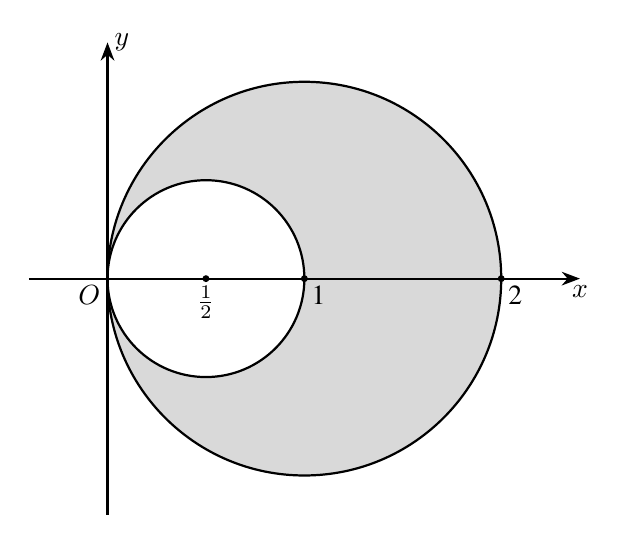
\begin{tikzpicture}[thick,inner sep=2.2pt,scale=2.5,>=Stealth]
  \filldraw [fill=gray!30,draw=black] (1,0) circle (1);
  \fill [white] (0.5,0) circle (0.5);
  \draw (0.5,0) circle (0.5);
  \draw [->] (-0.4,0) -- (0,0) node[below left]{$O$} -- (2.4,0) node [below]{$x$};
  \draw [->] (0,-1.2) -- (0,1.2) node [right]{$y$};
  \fill (0.5,0) node [below]{$\frac12$} circle(0.5pt)
  (1,0) node[below right]{1} circle(0.5pt)
  (2,0) node[below right]{2} circle(0.5pt);
\end{tikzpicture}
  \end{center}
  两个圆的极坐标方程分别为$r=\cos\theta$和$r=2\cos\theta$. 于是在极坐标系下,二重积分化为
  \begin{align*}
    I = \int_{-\frac\pi2}^{\frac\pi2}\mathrm d\theta
    \int_{\cos\theta}^{2\cos\theta}\sqrt{\frac{r^2-r\cos\theta}{2r\cos\theta-r^2}}r\mathrm dr
    = 2\int_0^{\frac\pi2}\mathrm d\theta
    \int_{\cos\theta}^{2\cos\theta}
    \sqrt{\frac{r-\cos\theta}{2\cos\theta-r}}r \mathrm dr
  \end{align*}
  令$a=\cos\theta,b=2\cos\theta$,注意到$r-a+b-r=b-a=a$,于是可令$r-a=a\sin^2t,b-r=a\cos^2t$,我们有
  \begin{align*}
    \int_a^b r\sqrt{\frac{r-a}{b-r}}\mathrm dr
    & = \int_0^{\frac\pi2}\big( a + a\sin^2t \big)\frac{\sin t}{\cos t}\cdot 2a\sin t\cos t\mathrm dt\\
    & = 2a^2 \int_0^{\frac\pi2} (\sin^2t + \sin^4t)\mathrm dt\\
    & = \frac{7\pi}8a^2= \frac{7\pi}8\cos^2\theta.
  \end{align*}
  于是
  \[
    I = 2\int_0^{\frac\pi2} \frac{7\pi}8\cos^2\theta \mathrm d\theta = \frac7{16}\pi^2.
  \]
\end{solve}

\end{MYBOX}

\end{document}

